\section{Numerical examples} 
\label{Sec1:resultsDisc}
To give further evidence for the correctness of the implemented code, comparison to existing benchmark solutions by Chang~\cite{Chang1994soa}, Ihlenburg~\cite{Ihlenburg1998fea} and Fender~\cite{Fender1972sfa}, will be presented. A final benchmark problem in the time-domain will be added.

It is customary to present results in the \textit{far-field}. For the scattered pressure $p_1$, it is defined by
\begin{equation}
	p_0(\hat{\vec{x}},\omega) =  r \euler^{-\imag k_1 r}p_1(\vec{x},\omega),\quad r = |\vec{x}| \to \infty,
\end{equation}
with $\hat{\vec{x}} = \vec{x}/|\vec{x}|$. As a side note, using \Cref{Eq1:sphericalHankelLimit}, the far-field pattern of the scattered pressure in \Cref{Eq1:outerFluid}, is given by (in the axisymmetric case)
\begin{equation}
	p_0 = \frac{1}{k_1}\sum_{n=0}^\infty \imag^{-n-1} Q_n^{(0)}(\vartheta) C_{1,n}^{(1)}
\end{equation}
which yields a very efficient way of computing the far-field pattern.

From the far-field pattern, the \textit{target strength}, $\TS$, can be computed. It is defined by
\begin{equation}\label{Eq1:TS}
	\TS = 20\log_{10}\left(\frac{|p_0(\hat{\vec{x}},\omega)|}{|P_{\mathrm{inc}}(\omega)|}\right)
\end{equation}
where $P_{\mathrm{inc}}$ is the amplitude of the incident wave at the geometric center of the scatterer (i.e. the origin). Note that $\TS$ is independent of $P_{\mathrm{inc}}$.

The directional vector, $\vec{d}_{\mathrm{s}}$, in spherical coordinates, is given by
\begin{equation}
	\vec{d}_{\mathrm{s}} = -\begin{bmatrix}
		\sin\vartheta_{\mathrm{s}}\cos\varphi_{\mathrm{s}}\\
		\sin\vartheta_{\mathrm{s}}\sin\varphi_{\mathrm{s}}\\
		\cos\vartheta_{\mathrm{s}}		
	\end{bmatrix}.
\end{equation}
If the source of the incident wave is located at
\begin{equation}\label{Eq1:x_s}
	\vec{x}_{\mathrm{s}} = -r_{\mathrm{s}}\vec{d}_{\mathrm{s}},
\end{equation}
the far-field pattern of an incident wave from the point source
\begin{equation}
	p_{\mathrm{inc}}(\vec{x},\omega) = P_{\mathrm{inc}}(\omega)\frac{\euler^{\imag k_1 |\vec{x}_{\mathrm{s}}-\vec{x}|}}{|\vec{x}_{\mathrm{s}}-\vec{x}|},
\end{equation}
is actually a plane wave
\begin{equation}
	\lim_{r_{\mathrm{s}}\to\infty} r_{\mathrm{s}}\euler^{-\imag k_1 r_{\mathrm{s}}}p_{\mathrm{inc}}(\vec{x},\omega) = P_{\mathrm{inc}}(\omega)\euler^{\imag k_1\vec{d}_{\mathrm{s}}\cdot\vec{x}}.
\end{equation}
Unless stated otherwise, plane waves will be used for the incident wave. Note that the direction of plane waves and location of far-field points is often expressed in the \textit{aspect angle}, $\alpha=\varphi$, and the \textit{elevation angle}, $\beta=\ang{90}-\vartheta$.

\subsection{Chang benchmark problem} 
Chang~\cite{Chang1994soa} considers a single spherical shell, with a single homogeneous Neumann condition (sound-soft boundary conditions, SSBC) on the inside of the shell, scattering an incident plane wave (with amplitude $P_{\mathrm{inc}}=\SI{1}{Pa}$). Chang sends the incident plane wave along the positive $x_3$-axis, and uses the parameters in \Cref{Tab1:Chang}.
\begin{table}
	\centering
	\caption{\textbf{Chang parameters:} Parameters for the examples in figure 16 and figure 17 in \cite{Chang1994soa}.}
	\label{Tab1:Chang}
	\begin{tabular}{l l}
		\toprule
		Parameter & Description\\
		\midrule
		$E = \SI{2.0e11}{Pa}$ & Young's modulus\\
		$\nu = 0.3$ & Poisson's ratio\\
		$\rho_{\mathrm{s}} = \SI{7800}{kg.m^{-3}}$ & Density of solid\\
		$\rho_{\mathrm{f}} = \SI{1000}{kg.m^{-3}}$ & Density of water\\
		$c_{\mathrm{f},1} = \SI{1460}{m.s^{-1}}$ & Speed of sound in fluid\\
		$R_{0,1} = \SI{1.005}{m}$ & Outer radius of spherical shell\\
		$R_{1,1} = \SI{0.995}{m}$ & Inner radius of spherical shell\\
		\bottomrule
	\end{tabular}
\end{table}
Moreover, the total pressure (\Cref{Eq1:totPressure}) is measured at the surface. In \Cref{Fig1:Chang1,Fig1:Chang2} the results are found with $k=\SI{15}{m^{-1}}$ and $k=\SI{20}{m^{-1}}$, respectively\footnote{The discrepancies probably comes from the fact that the data set is collected by the software \href{https://automeris.io/WebPlotDigitizer/}{WebPlotDigitizer} where a digital scan of figure 16 and figure 17~\cite[pp. 32-33]{Chang1994soa} has been made.}. In both cases, the shadow region of the scatterer, $\vartheta\in [0,\ang{90}]$, is clearly visible (with total pressure significantly lower than $P_{\mathrm{inc}}$).
\begin{figure}
	\centering
	\begin{subfigure}[t]{\textwidth}
		\centering
		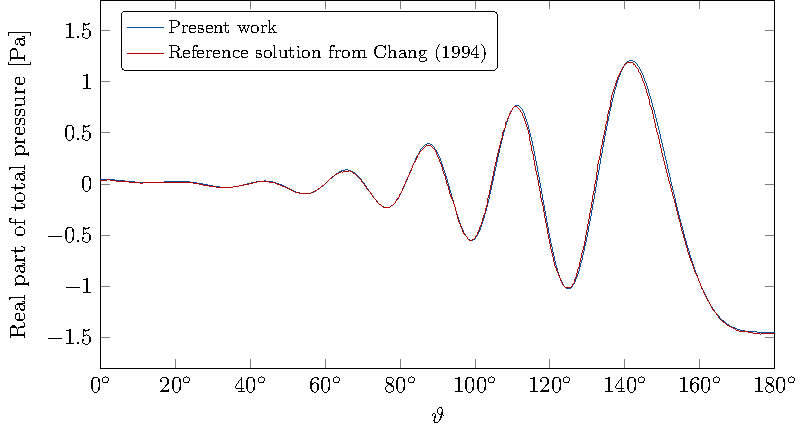
\includegraphics{../../LaTeX/createFigures/TikzFigures/article_e3Dss_PhD/Chang_BI_A0_Em90_1}
%		\includegraphics{\graphicsFolder/Figure7a}
		\caption{Wave number $k_1=\SI{15}{m^{-1}}$ and series truncation at $N_\varepsilon = 46$.}
		\label{Fig1:Chang1}
	\end{subfigure}
	\par\bigskip
	\begin{subfigure}[t]{\textwidth}
		\centering
		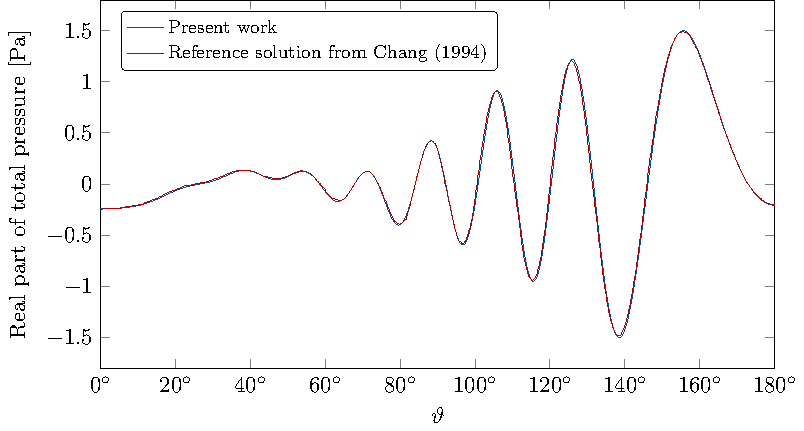
\includegraphics{../../LaTeX/createFigures/TikzFigures/article_e3Dss_PhD/Chang_BI_A0_Em90_2}
%		\includegraphics{\graphicsFolder/Figure7b}
		\caption{Wave number $k_1=\SI{20}{m^{-1}}$ and series truncation at $N_\varepsilon = 54$.}
		\label{Fig1:Chang2}
	\end{subfigure}
	\caption{\textbf{Chang benchmark problem}: Predicted total pressure as a function of the polar angle $\vartheta$.}
\end{figure}

A simple convergence analysis is shown in \Cref{Fig1:ChangErrors} where the error in the truncated series in \Cref{Eq1:truncated_p1} is plotted. As discussed in \Cref{Subsec1:seriesEval} the convergence is delayed by the increased frequency from $k_1=\SI{15}{m^{-1}}$ to $k_1=\SI{20}{m^{-1}}$. To obtain machine epsilon precision (double precision) $N_\varepsilon=45$ and $N_\varepsilon=53$ is needed for these frequencies, respectively.
\begin{figure}
	\centering
	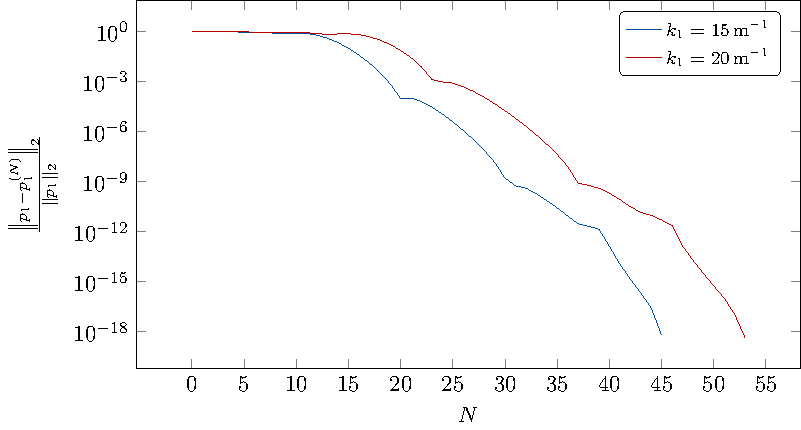
\includegraphics{../../LaTeX/createFigures/TikzFigures/article_e3Dss_PhD/Chang_Errors}
%	\includegraphics{\graphicsFolder/Figure8}
	\caption{\textbf{Chang benchmark problem}: Relative error (with 2000 sample points uniformly placed in the $\vartheta$-direction) of the truncated series in \Cref{Eq1:truncated_p1} as a function of $N$.}
	\label{Fig1:ChangErrors}
\end{figure}

\subsection{Ihlenburg benchmark problem} 
Ihlenburg~\cite{Ihlenburg1998fea} considers a single spherical shell with a single homogeneous Neumann condition (sound-soft boundary conditions, SSBC) on the inside of the shell, scattering an incident plane wave. 

Building upon this example, the corresponding rigid scattering (sound-hard boundary conditions, SHBC) case and scattering with fluid fill will be presented (Neumann-Neumann boundary conditions, NNBC). The parameters in \Cref{Tab1:IhlenburgParameters} are here used. 

Frequency sweeps of the target strength (in \Cref{Eq1:TS}) are plotted in \Cref{Fig1:Fender1,Fig1:Fender2} at the polar angles $\vartheta=\ang{180}$ and $\vartheta=\ang{0}$, respectively.
\begin{table}
	\centering
	\caption{\textbf{Ihlenburg parameters:} Parameters for the Ihlenburg benchmark problem.}
	\label{Tab1:IhlenburgParameters}
	\begin{tabular}{l l}
		\toprule
		Parameter & Description\\
		\midrule
		$E = \SI{2.07e11}{Pa}$ & Young's modulus\\
		$\nu = 0.3$ & Poisson's ratio\\
		$\rho_{\mathrm{s}} = \SI{7669}{kg.m^{-3}}$ & Density of solid\\
		$\rho_{\mathrm{f}} = \SI{1000}{kg.m^{-3}}$ & Density of water\\
		$c_{\mathrm{f}} = \SI{1524}{m.s^{-1}}$ & Speed of sound in fluid\\
		$R_{0,1}=\SI{5.075}{m}$ & Outer radius\\
		$R_{1,1}=\SI{4.925}{m}$ & Inner radius\\
		\bottomrule
	\end{tabular}
\end{table}

\begin{figure}
	\centering
	\begin{subfigure}[t]{\textwidth}
		\centering
		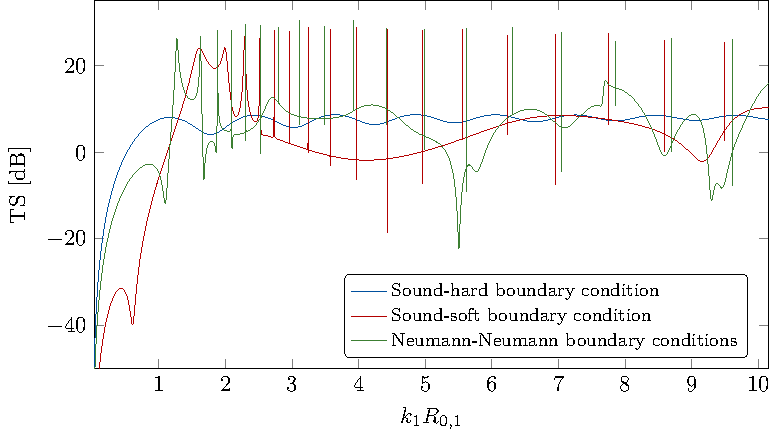
\includegraphics{../../LaTeX/createFigures/TikzFigures/article_e3Dss_PhD/IL_Sweep_A180_E0_FS_1}
%		\includegraphics{\graphicsFolder/Figure9a}
		\caption{Measured at $\vartheta = \ang{180}$.}
		\label{Fig1:Ihlenburg1}
	\end{subfigure}
	\par\bigskip
	\begin{subfigure}[t]{\textwidth}
		\centering
		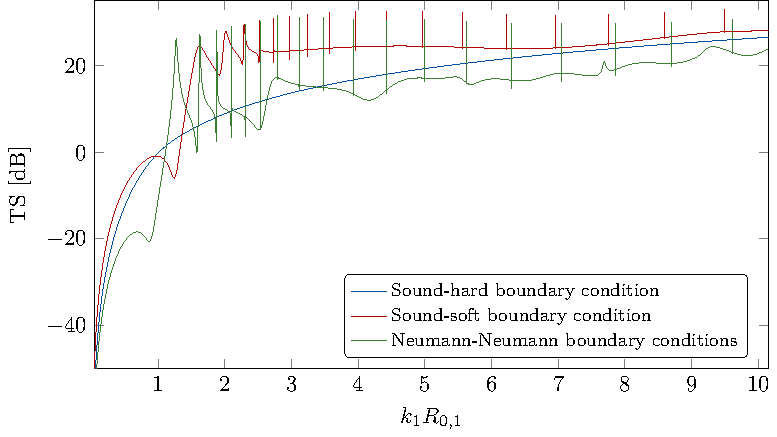
\includegraphics{../../LaTeX/createFigures/TikzFigures/article_e3Dss_PhD/IL_Sweep_A180_E0_FS_2}
%		\includegraphics{\graphicsFolder/Figure9b}
		\caption{Measured at $\vartheta = \ang{0}$.}
		\label{Fig1:Ihlenburg2}
	\end{subfigure}
	\caption{\textbf{Ihlenburg benchmark problem}: Plots of the target strength, $\TS$. The backscattered pressure will correspond to $\vartheta=\ang{180}$, which is also the specific case considered by Ihlenburg \cite[p. 192]{Ihlenburg1998fea} (note that Ihlenburg plots the far field instead of the target strength).}
\end{figure}
Convergence plots for the three different cases are plotted in \Cref{Fig1:IhlenburgErrors1,Fig1:IhlenburgErrors2,Fig1:IhlenburgErrors3}, respectively. The linear computational complexity discussed in \Cref{Subsec1:seriesEval} is revealed. Moreover, by comparing the SHBC case in \Cref{Fig1:IhlenburgErrors1} to the SSBC and NNBC cases in \Cref{Fig1:IhlenburgErrors2,Fig1:IhlenburgErrors3}, it is clear that the eigenmodes requires more terms (larger $N$) in order to achieve better than 1\% error precision (this is in particular the case for eigenmodes at higher frequencies). 

However, the eigenmodes has no need of more terms in order to reach machine epsilon precision. So in the case of elastic scattering, the series termination strategy described in \Cref{Subsec1:seriesEval} is more rigorous than termination of the series at a given $N$ linearly depending on the frequency.
\begin{figure}
	\centering
	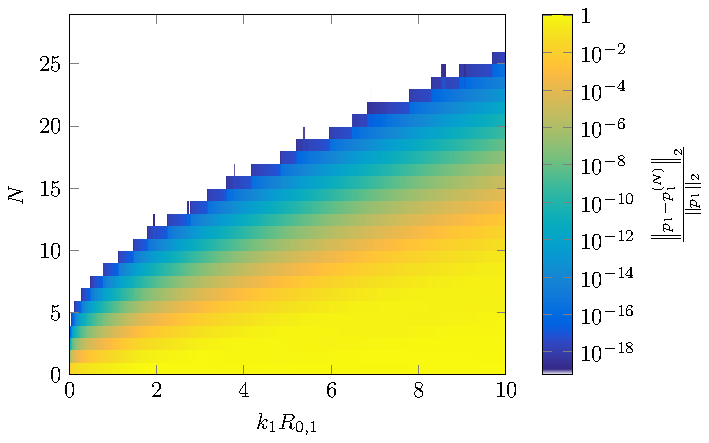
\includegraphics{../../LaTeX/createFigures/TikzFigures/article_e3Dss_PhD/IhlenburgErrors_1}
%	\includegraphics{\graphicsFolder/Figure10}
		\caption{\textbf{Ihlenburg benchmark problem - the sound-hard case}: Relative error in the $l_2$-norm (with two sample points at $\vartheta = \ang{0}$ and $\vartheta = \ang{180}$) of the truncated series in \Cref{Eq1:truncated_p1} as a function of $N$. The ``exact'' solution, $p_1$, is obtained as described in \Cref{Subsec1:seriesEval}.}
	\label{Fig1:IhlenburgErrors1}
\end{figure}
\begin{figure}
	\centering
	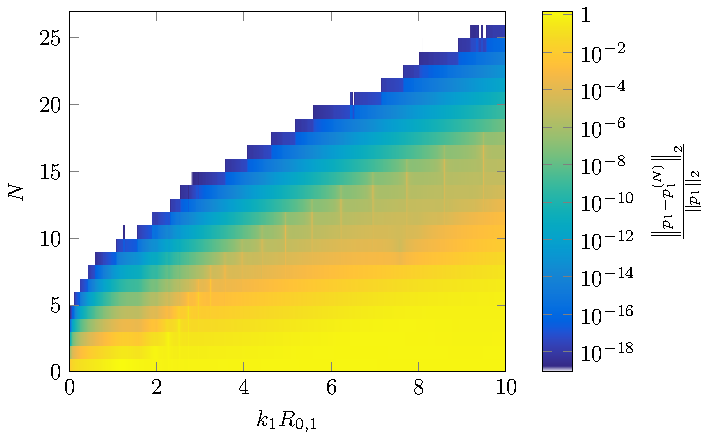
\includegraphics{../../LaTeX/createFigures/TikzFigures/article_e3Dss_PhD/IhlenburgErrors_2}
%	\includegraphics{\graphicsFolder/Figure11}
		\caption{\textbf{Ihlenburg benchmark problem - the sound-soft case}: Relative error in the $l_2$-norm (with two sample points at $\vartheta = \ang{0}$ and $\vartheta = \ang{180}$) of the truncated series in \Cref{Eq1:truncated_p1} as a function of $N$. The ``exact'' solution, $p_1$, is obtained as described in \Cref{Subsec1:seriesEval}.}
	\label{Fig1:IhlenburgErrors2}
\end{figure}
\begin{figure}
	\centering
	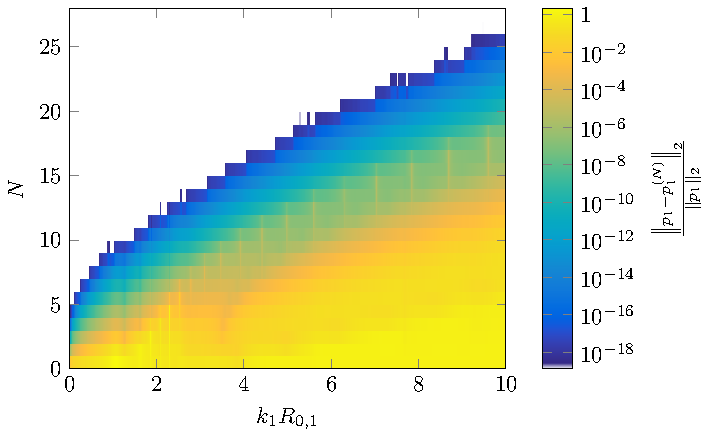
\includegraphics{../../LaTeX/createFigures/TikzFigures/article_e3Dss_PhD/IhlenburgErrors_3}
%	\includegraphics{\graphicsFolder/Figure12}
		\caption{\textbf{Ihlenburg benchmark problem - the Neumann-Neumann case}: Relative error in the $l_2$-norm (with two sample points at $\vartheta = \ang{0}$ and $\vartheta = \ang{180}$) of the truncated series in \Cref{Eq1:truncated_p1} as a function of $N$. The ``exact'' solution, $p_1$, is obtained as described in \Cref{Subsec1:seriesEval}.}
	\label{Fig1:IhlenburgErrors3}
\end{figure}

\subsection{Fender benchmark problem} 
Fender~\cite{Fender1972sfa} consider a single air-filled spherical shell scattering an incident plane wave (with amplitude $P_{\mathrm{inc}}=\SI{1}{Pa}$). The parameters in \Cref{Tab1:Fender} are here used,
\begin{table}
	\centering
	\caption{\textbf{Fender parameters:} Parameters for the examples in figure 2 and figure 3 in \cite{Fender1972sfa}.}
	\label{Tab1:Fender}
	\begin{tabular}{l l}
		\toprule
		Parameter & Description\\
		\midrule
		$c_{\mathrm{s},1} = \SI{6412}{m.s^{-1}}$ & Longitudinal wave velocity\\
		$c_{\mathrm{s},2} = \SI{3043}{m.s^{-1}}$ & Transverse wave velocity\\
		$\rho_{\mathrm{s},1} = \SI{2700}{kg.m^{-3}}$ & Density of solid\\
		$\rho_{\mathrm{f},1} = \SI{1026}{kg.m^{-3}}$ & Density of outer fluid (water)\\
		$\rho_{\mathrm{f},2} = \SI{1.21}{kg.m^{-3}}$ & Density of inner fluid (air)\\
		$c_{\mathrm{f},1} = \SI{1500}{m.s^{-1}}$ & Speed of sound in water\\
		$c_{\mathrm{f},2} = \SI{343}{m.s^{-1}}$ & Speed of sound in air\\
		$R_{0,1} = \SI{1}{m}$ & Outer radius of spherical shell\\
		$R_{1,1} = \SI{0.95}{m}$ & Inner radius of spherical shell\\
		\bottomrule
	\end{tabular}
\end{table}
where the following conversion formulas is of convenience
\begin{equation}
	E = \rho_s c_{\mathrm{s},2}^2\frac{3c_{\mathrm{s},1}^2-4c_{\mathrm{s},2}^2}{c_{\mathrm{s},1}^2-c_{\mathrm{s},2}^2}\quad\text{and}\quad
	\nu = \frac12 \frac{c_{\mathrm{s},1}^2-2c_{\mathrm{s},2}^2}{c_{\mathrm{s},1}^2-c_{\mathrm{s},2}^2}.
\end{equation}
Fender also sends the incident plane wave along the $x_3$-axis, but in negative direction. The frequency sweep results of the total pressure (in \Cref{Eq1:totPressure}) are measured at the surface. In \Cref{Fig1:Fender1,Fig1:Fender2} the results are found at polar angles $\vartheta=\ang{0}$ and $\vartheta=\ang{180}$, respectively\footnote{The discrepancies again probably comes from the fact that the data set is collected by the software \href{https://automeris.io/WebPlotDigitizer/}{WebPlotDigitizer} where a digital scan of Figure 2 and Figure 3~\cite[pp. 30-31]{Fender1972sfa} has been made. Moreover, the spectrum has been sampled rather closely, revealing small (less significant) eigenmodes not shown by Fender.}.
\begin{figure}
	\centering
	\begin{subfigure}[t]{\textwidth}
		\centering
		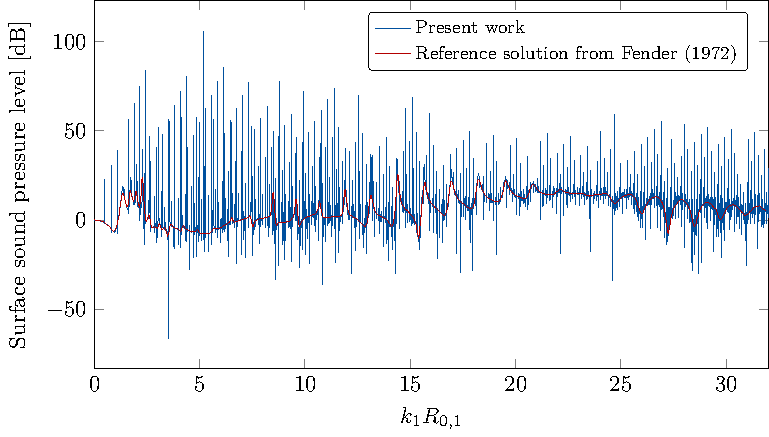
\includegraphics{../../LaTeX/createFigures/TikzFigures/article_e3Dss_PhD/Fender_Sweep_A0_E90_FS_1}
%	\includegraphics{\graphicsFolder/Figure13a}
		\caption{Measured at $\vartheta = \ang{0}$.}
		\label{Fig1:Fender1}
	\end{subfigure}
	\par\bigskip
	\begin{subfigure}[t]{\textwidth}
		\centering
		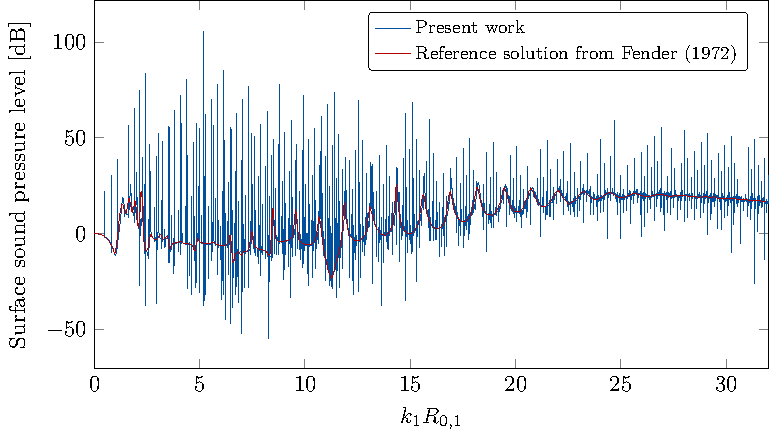
\includegraphics{../../LaTeX/createFigures/TikzFigures/article_e3Dss_PhD/Fender_Sweep_A0_E90_FS_2}
%	\includegraphics{\graphicsFolder/Figure13b}
		\caption{Measured at $\vartheta = \ang{180}$.}
		\label{Fig1:Fender2}
	\end{subfigure}
	\caption{\textbf{Fender benchmark problem}: Predicted total pressure as a function of $k_1R_{0,1}$ at the surface of the shell.}
\end{figure}

In \Cref{Fig1:FenderConvergence}, another convergence study is illustrated. The Fender benchmark problem was run with increasing frequency until a Bessel function was evaluated to be above $10^{290}$ (the termination criterion as described in \Cref{Subsec1:RoundoffErrors}). Due to the linear behavior of $N$ as a function of $\omega$ needed for convergence (computational complexity) and the concave behavior of the smallest number $N$ such that $|\bessely_N(\omega\Upsilon)|>10^{290}$ (where $\Upsilon$ is given by \Cref{Eq1:Upsilon}), prematurely termination of the series is inevitable for large enough frequencies.
\begin{figure}
	\centering
	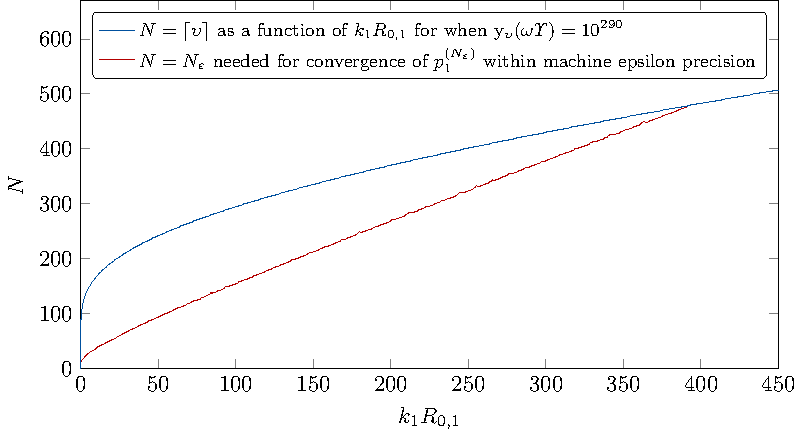
\includegraphics{../../LaTeX/createFigures/TikzFigures/article_e3Dss_PhD/Fender_bound}
%	\includegraphics{\graphicsFolder/Figure14}
		\caption{\textbf{Fender benchmark problem}: The intersection of these to graphs marks the largest frequency for which the algorithms presented in this work will give satisfactory results. Here, $\Upsilon$ is given by \Cref{Eq1:Upsilon} and the truncated series $p_1^{(N_\varepsilon)}$ is given by \Cref{Eq1:truncated_p1}.}
	\label{Fig1:FenderConvergence}
\end{figure}


\subsection{Benchmark problems}
\label{Subsec1:benchmarkProblem}
Let S1, S3 and S5 be benchmark models of spherical shells characterized by the outer radius $R_{0,1}$ and the inner radius $R_{1,1}$ of the shell. The shells are filled with the given fluid (\Cref{Tab1:S1S3S5}) and embedded in water.
\begin{table}
	\centering%
	\caption{\textbf{Benchmark problems:} Parameters for S1, S3 and S5.}
	\label{Tab1:S1S3S5}
	\begin{tabular}{l l l l}
		\toprule
		 & S1 & S3 & S5 \\
		\midrule
		Outer radius, $R_{0,1}$ & $\SI{1}{m}$ & $\SI{3}{m}$ & $\SI{5}{m}$\\
		Inner radius, $R_{1,1}$ & $\SI{0.95}{m}$ & $\SI{2.98}{m}$ & $\SI{4.992}{m}$\\
		Fluid fill & air & air & water\\
		\bottomrule
	\end{tabular}
\end{table}
The remaining parameters are given in \Cref{Tab1:sphericalShellParameters}. 
\begin{table}
	\centering
	\caption{\textbf{Benchmark problems:} Common parameters for the benchmark problems.}
	\label{Tab1:sphericalShellParameters}
	\begin{tabular}{l l}
		\toprule
		Parameter & Description\\
		\midrule
		$E = \SI{2.10e11}{Pa}$ & Young's modulus\\
		$\nu = 0.3$ & Poisson's ratio\\
		$\rho_{\mathrm{s}} = \SI{7850}{kg.m^{-3}}$ & Density of solid\\
		$\rho_{\mathrm{f,water}} = \SI{1000}{kg.m^{-3}}$ & Density of water\\
		$\rho_{\mathrm{f,air}} = \SI{1.2}{kg.m^{-3}}$ & Density of air\\
		$c_{\mathrm{f,water}} = \SI{1500}{m.s^{-1}}$ & Speed of sound in water\\
		$c_{\mathrm{f,air}} = \SI{340}{m.s^{-1}}$ & Speed of sound in air\\
		\bottomrule
	\end{tabular}
\end{table}
These models can be combined into a new set of benchmark problems: S13 (S1 inside S3 with air in between), S15 (S1 inside S5 with water in between), S35 (S3 inside S5 with water in between) and S135 (S1 inside S3 inside S5 with air in between S1 and S3 and water in between S3 and S5). These benchmark problems are illustrated in \Cref{Fig1:BenchmarksProblems}.
\begin{figure}
	\centering
	\begin{subfigure}{0.3\textwidth}
		\centering
%		\includegraphics[width=0.8\textwidth]{\graphicsFolder/Figure15a}
		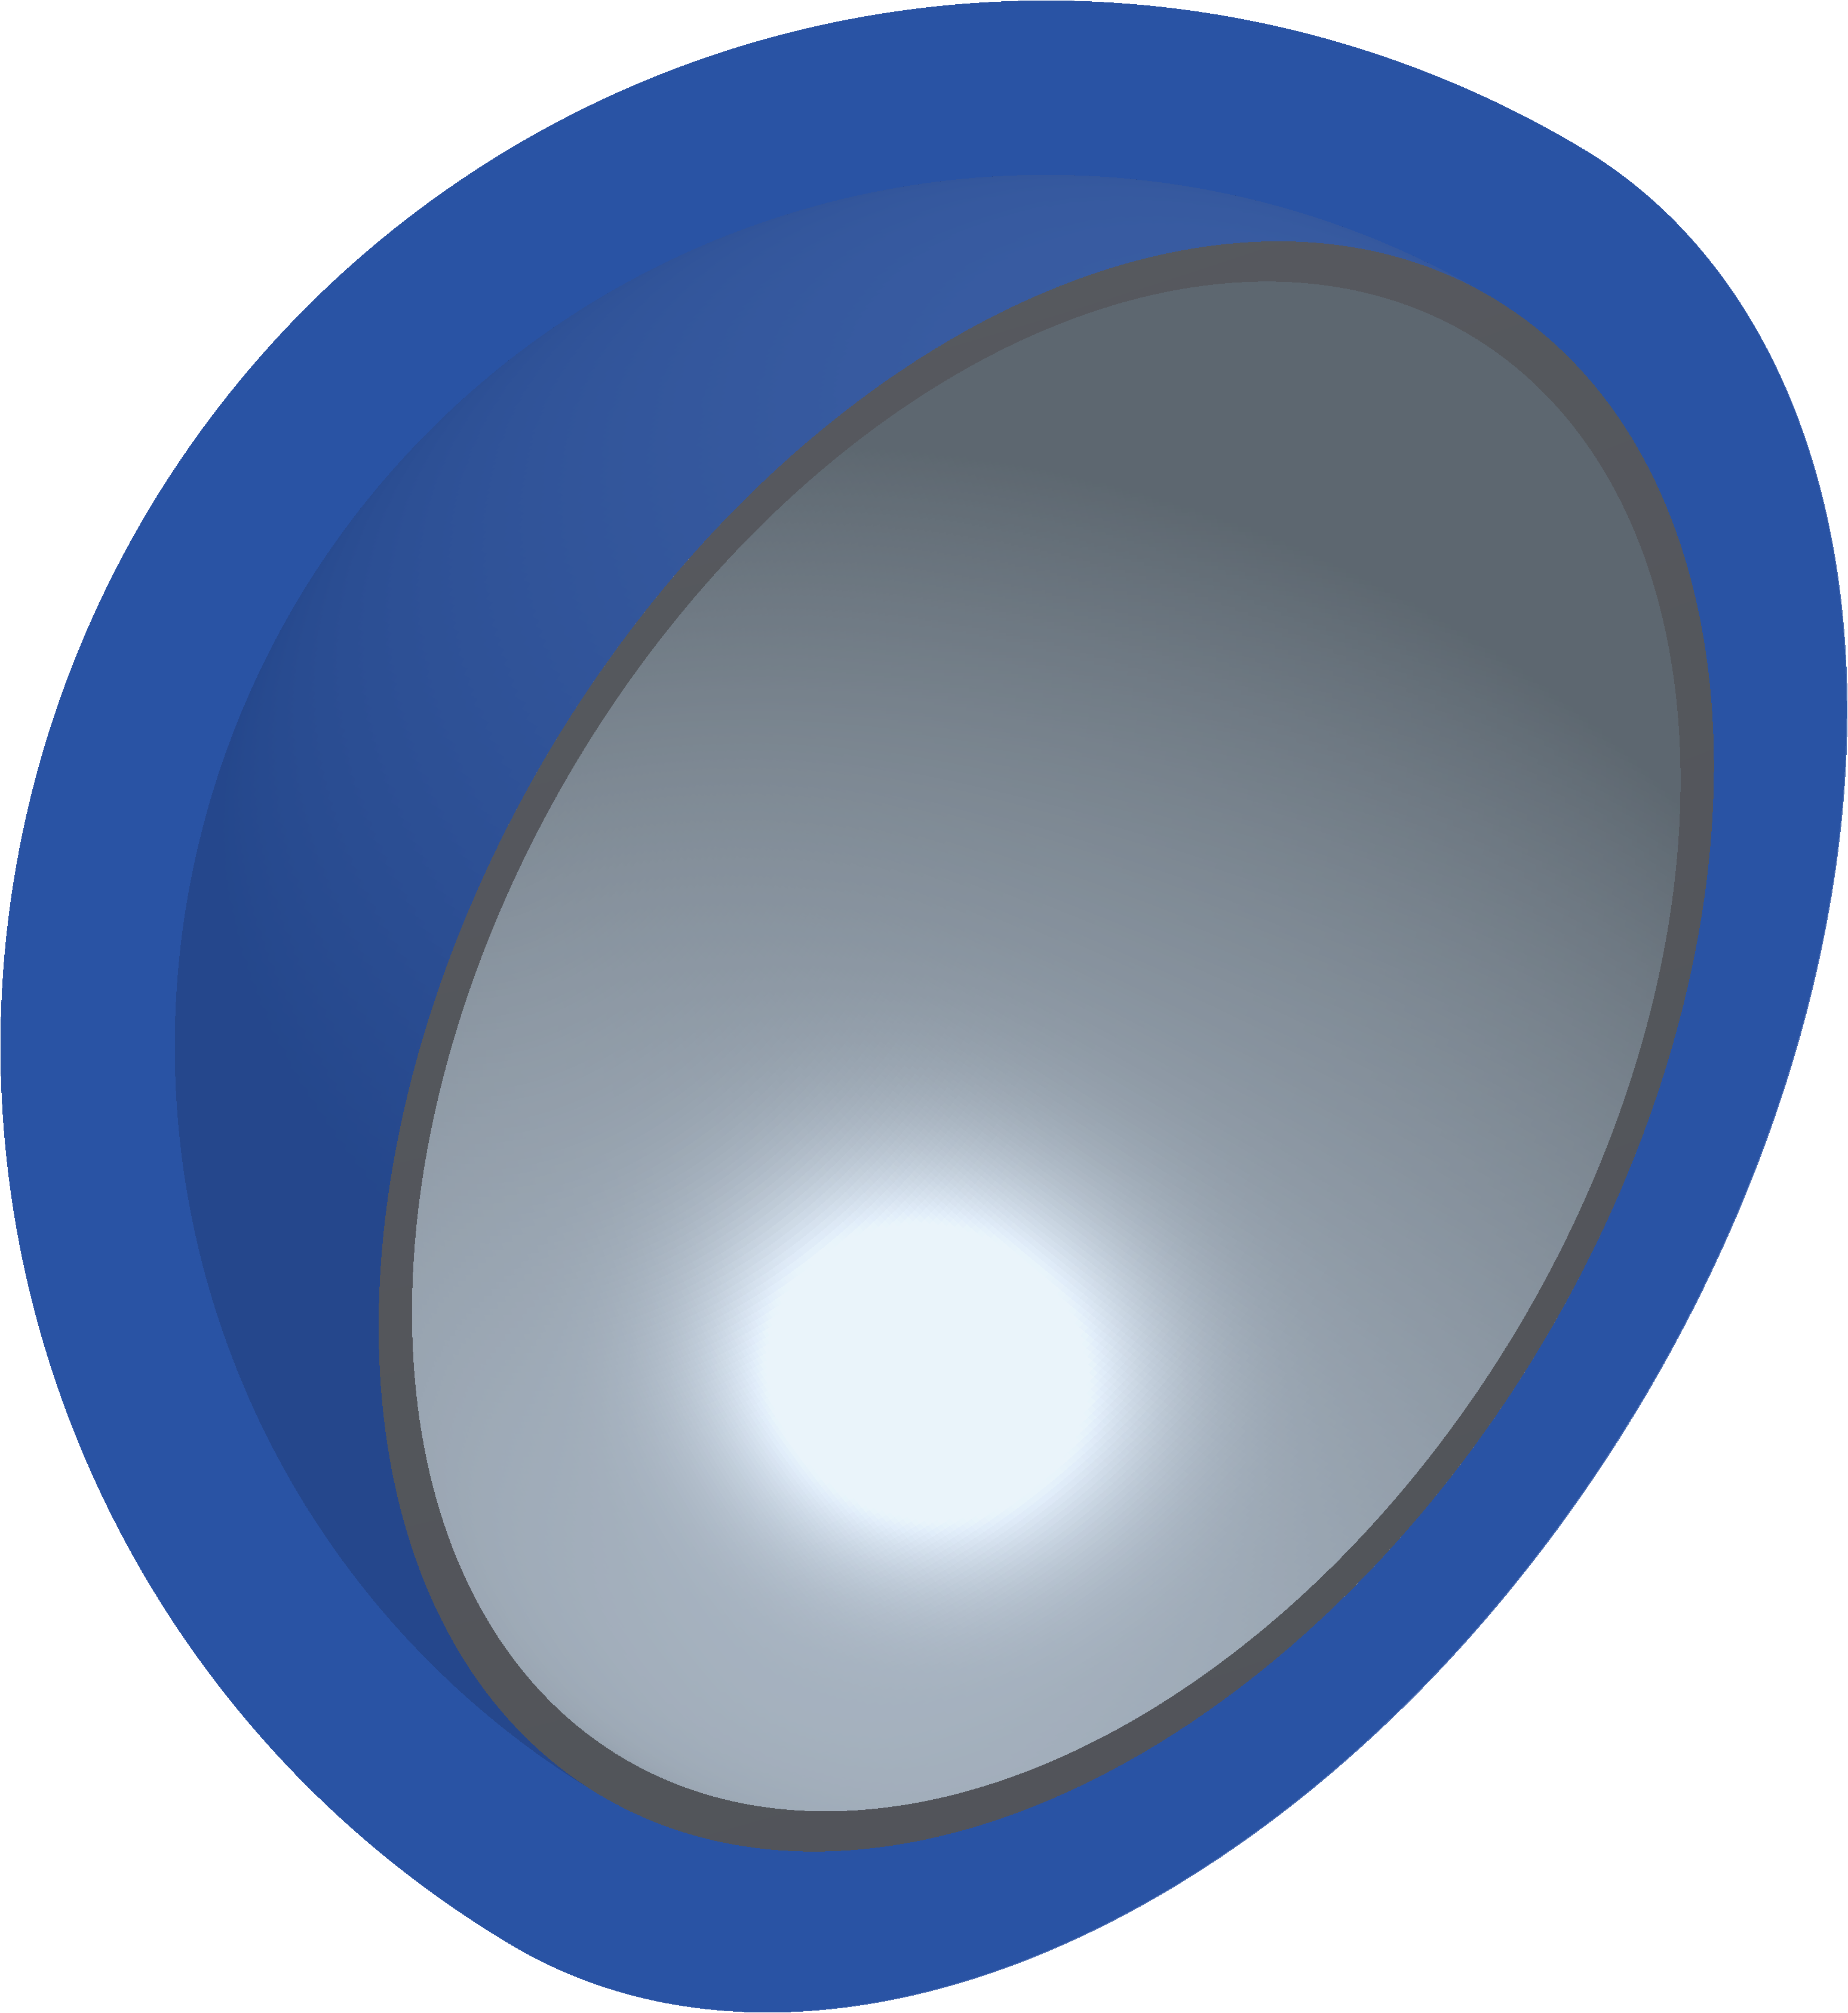
\includegraphics[width=0.8\textwidth]{../../graphics/sphericalShell/half_S1}
		\caption{S1}
    \end{subfigure}
	~
	\begin{subfigure}{0.3\textwidth}
		\centering
%		\includegraphics[width=0.8\textwidth]{\graphicsFolder/Figure15b}
		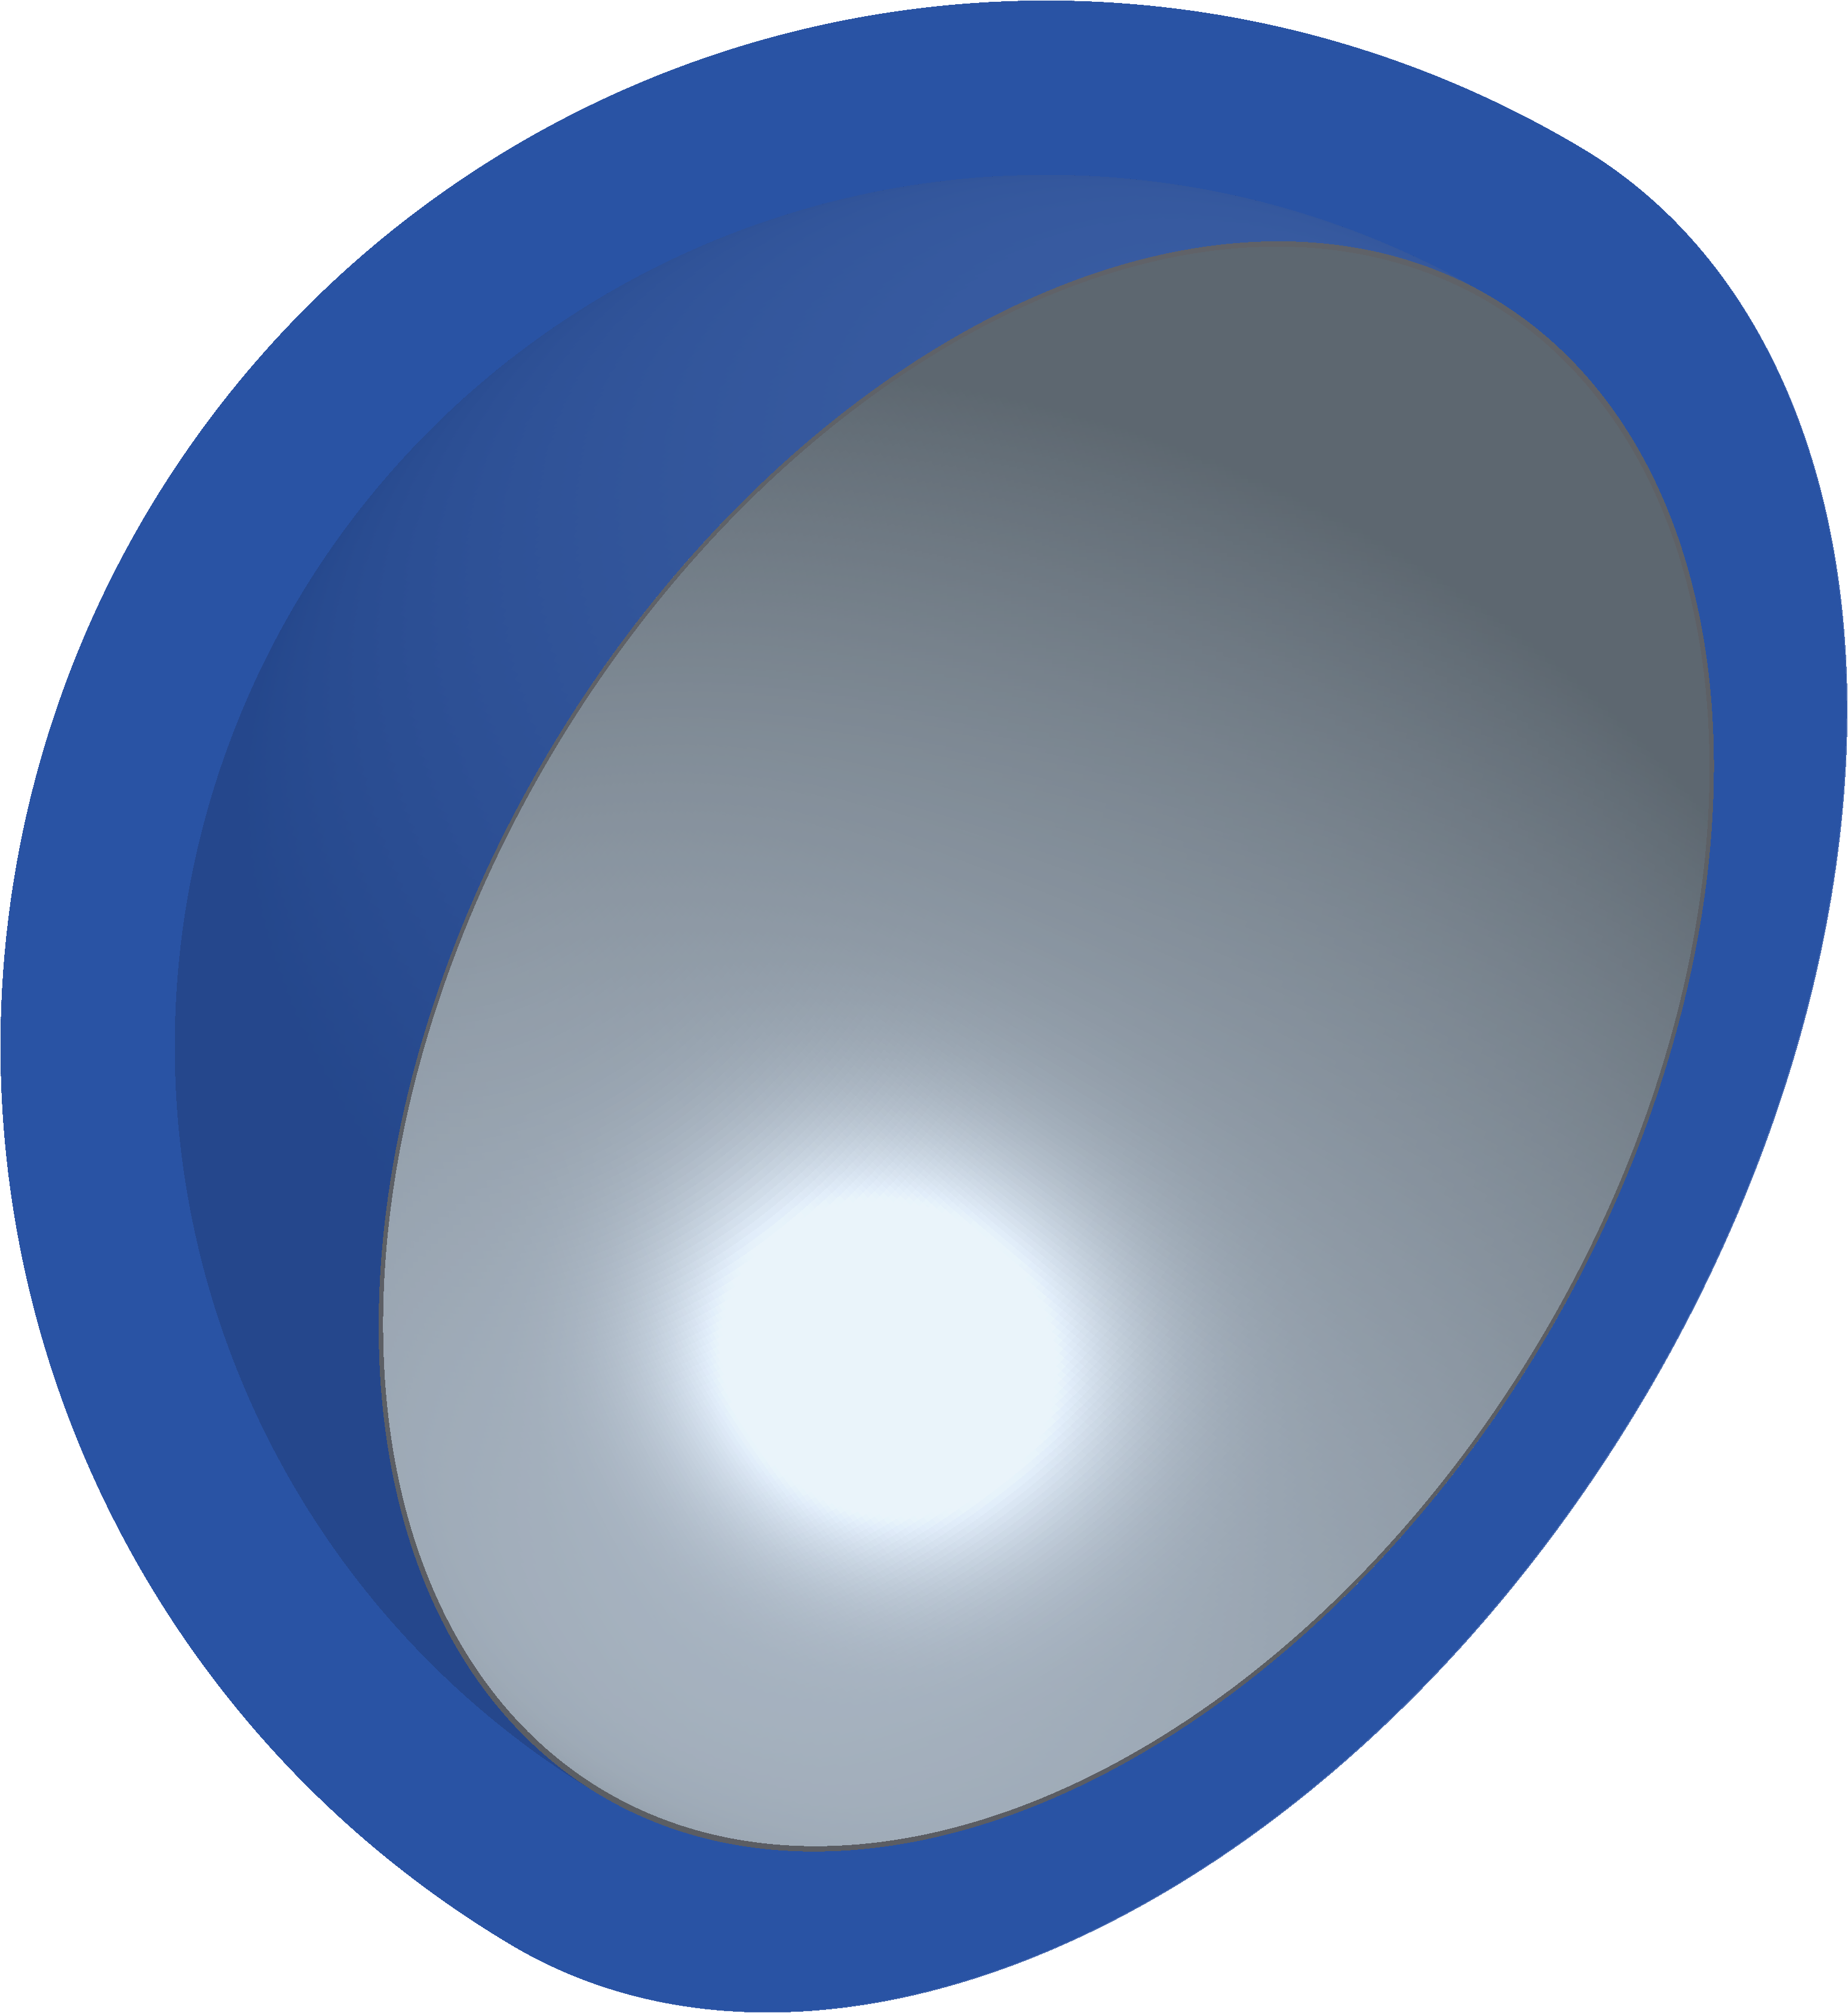
\includegraphics[width=0.8\textwidth]{../../graphics/sphericalShell/half_S3}
		\caption{S3}
    \end{subfigure}
	~
	\begin{subfigure}{0.3\textwidth}
		\centering
%		\includegraphics[width=0.8\textwidth]{\graphicsFolder/Figure15c}
		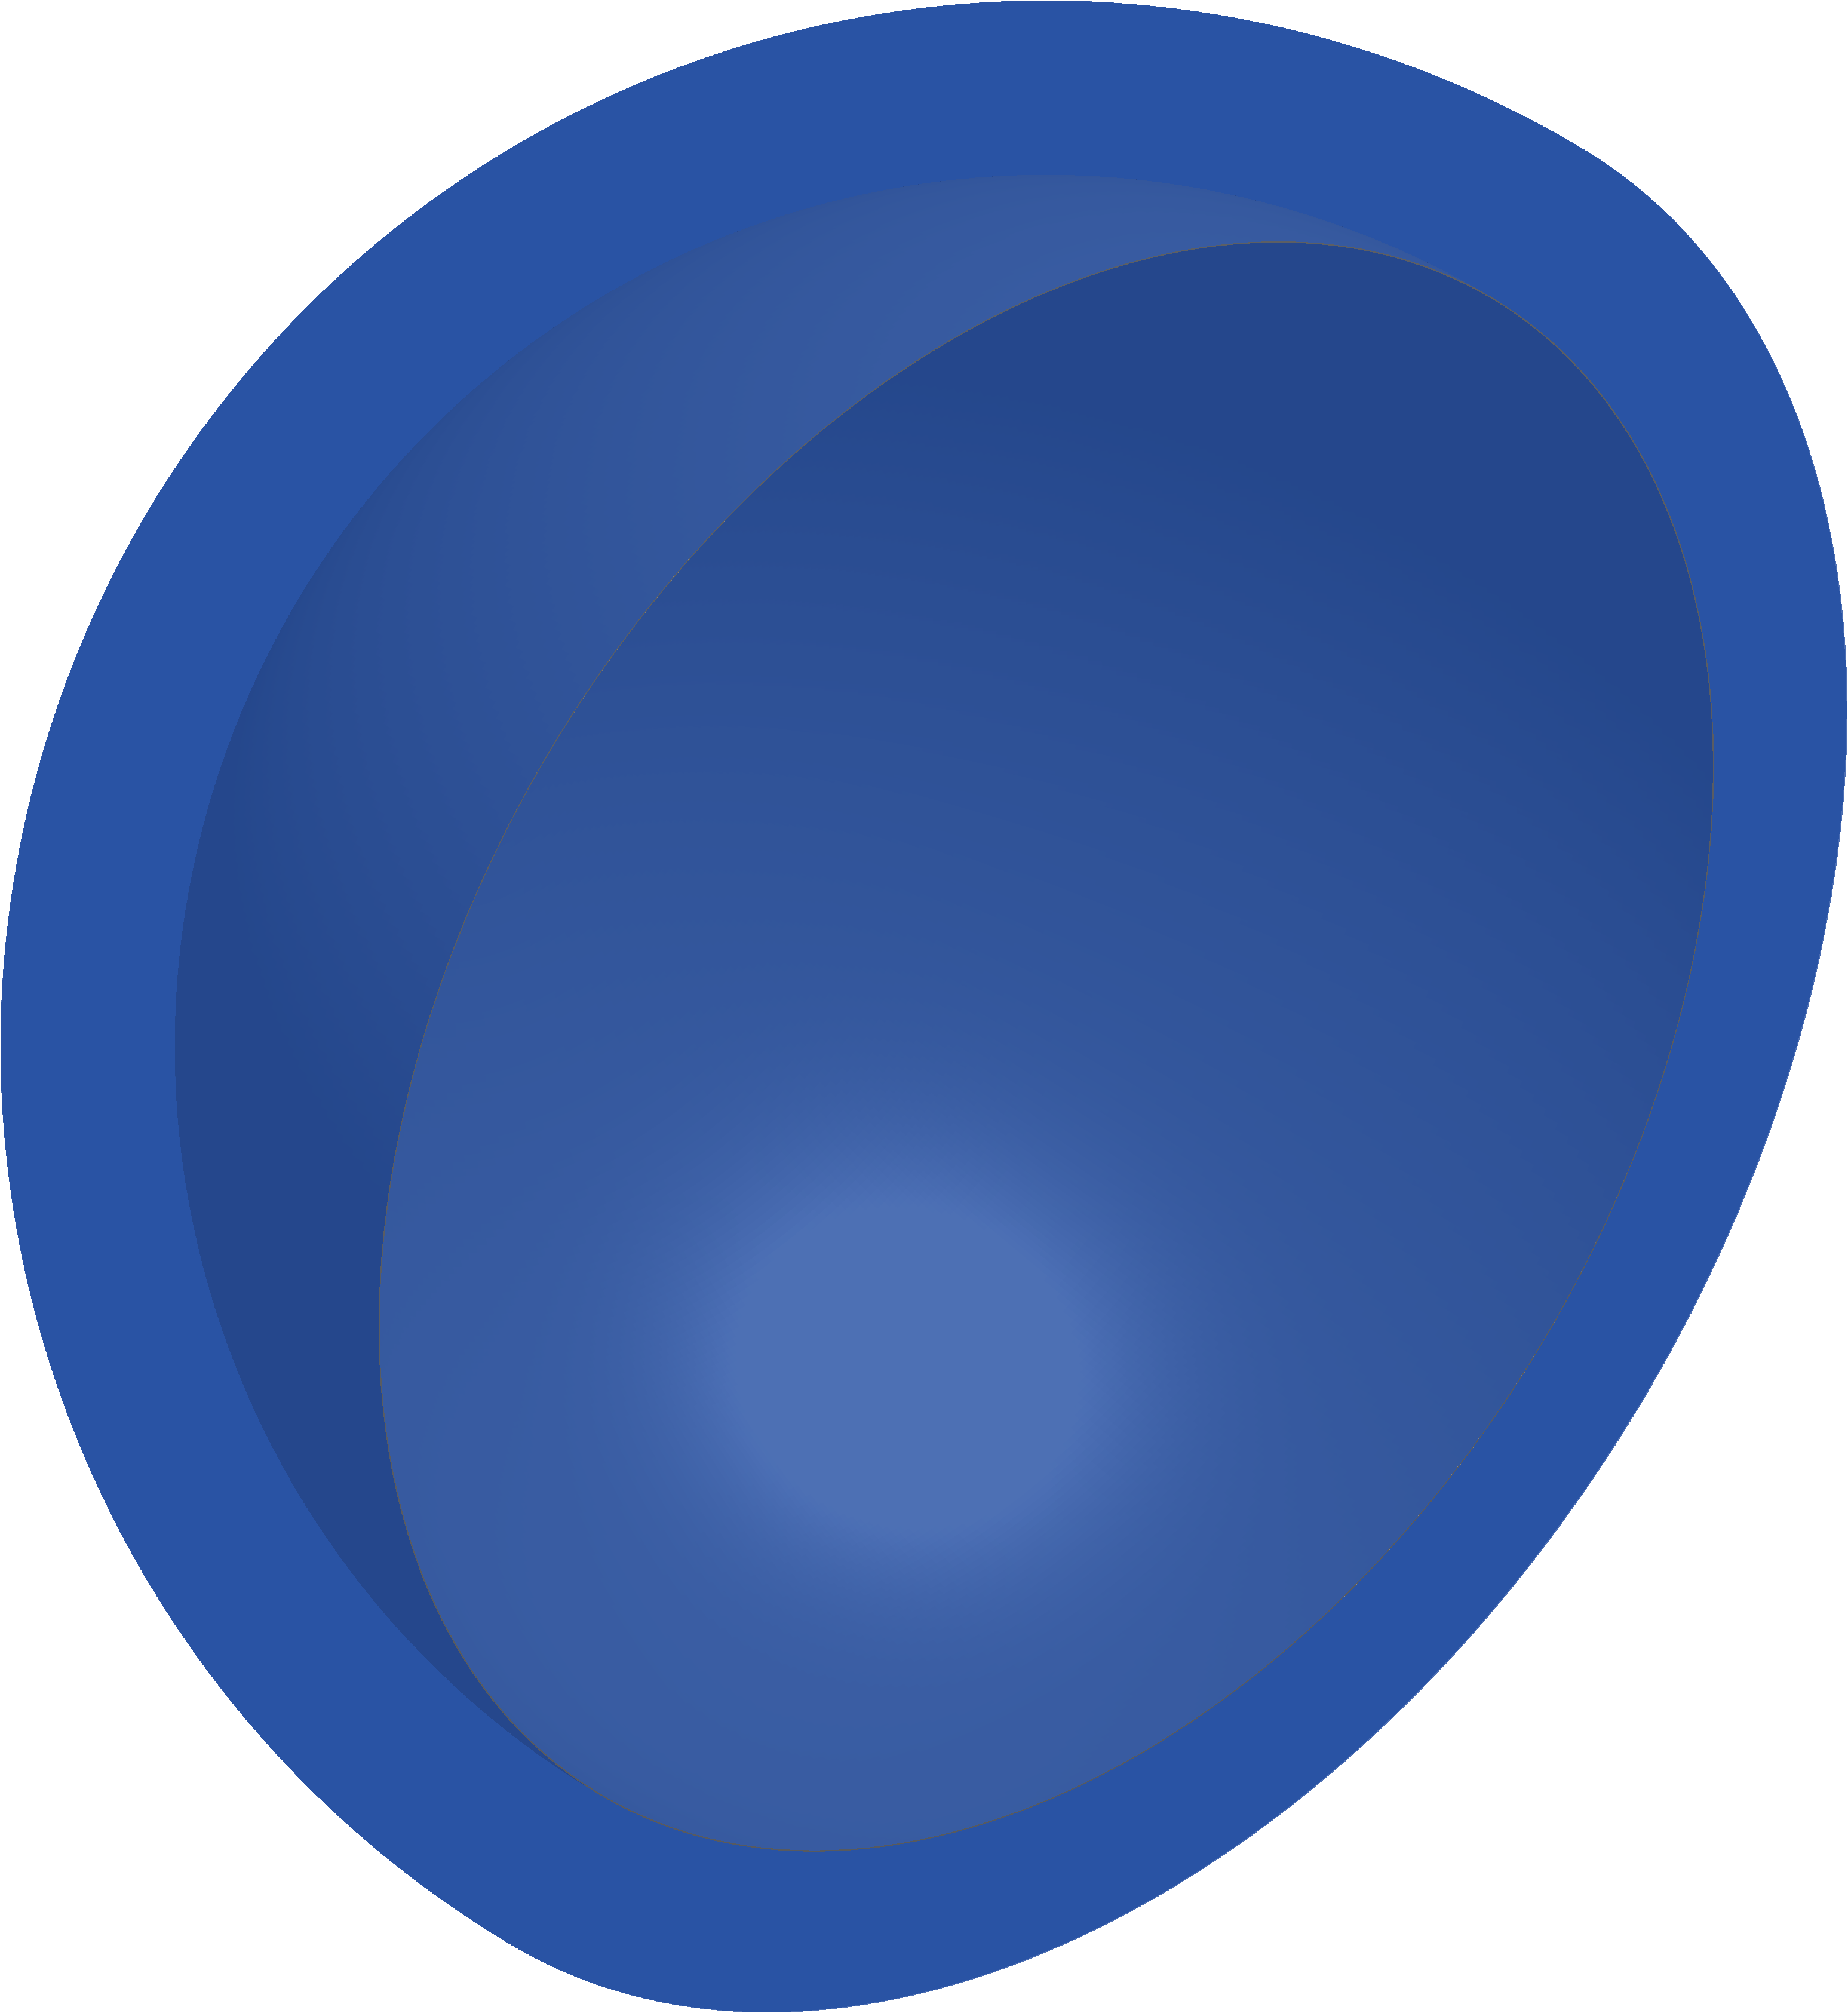
\includegraphics[width=0.8\textwidth]{../../graphics/sphericalShell/half_S5}
		\caption{S5}
    \end{subfigure}
	\par\bigskip
	\begin{subfigure}{0.3\textwidth}
		\centering
%		\includegraphics[width=0.8\textwidth]{\graphicsFolder/Figure15d}
		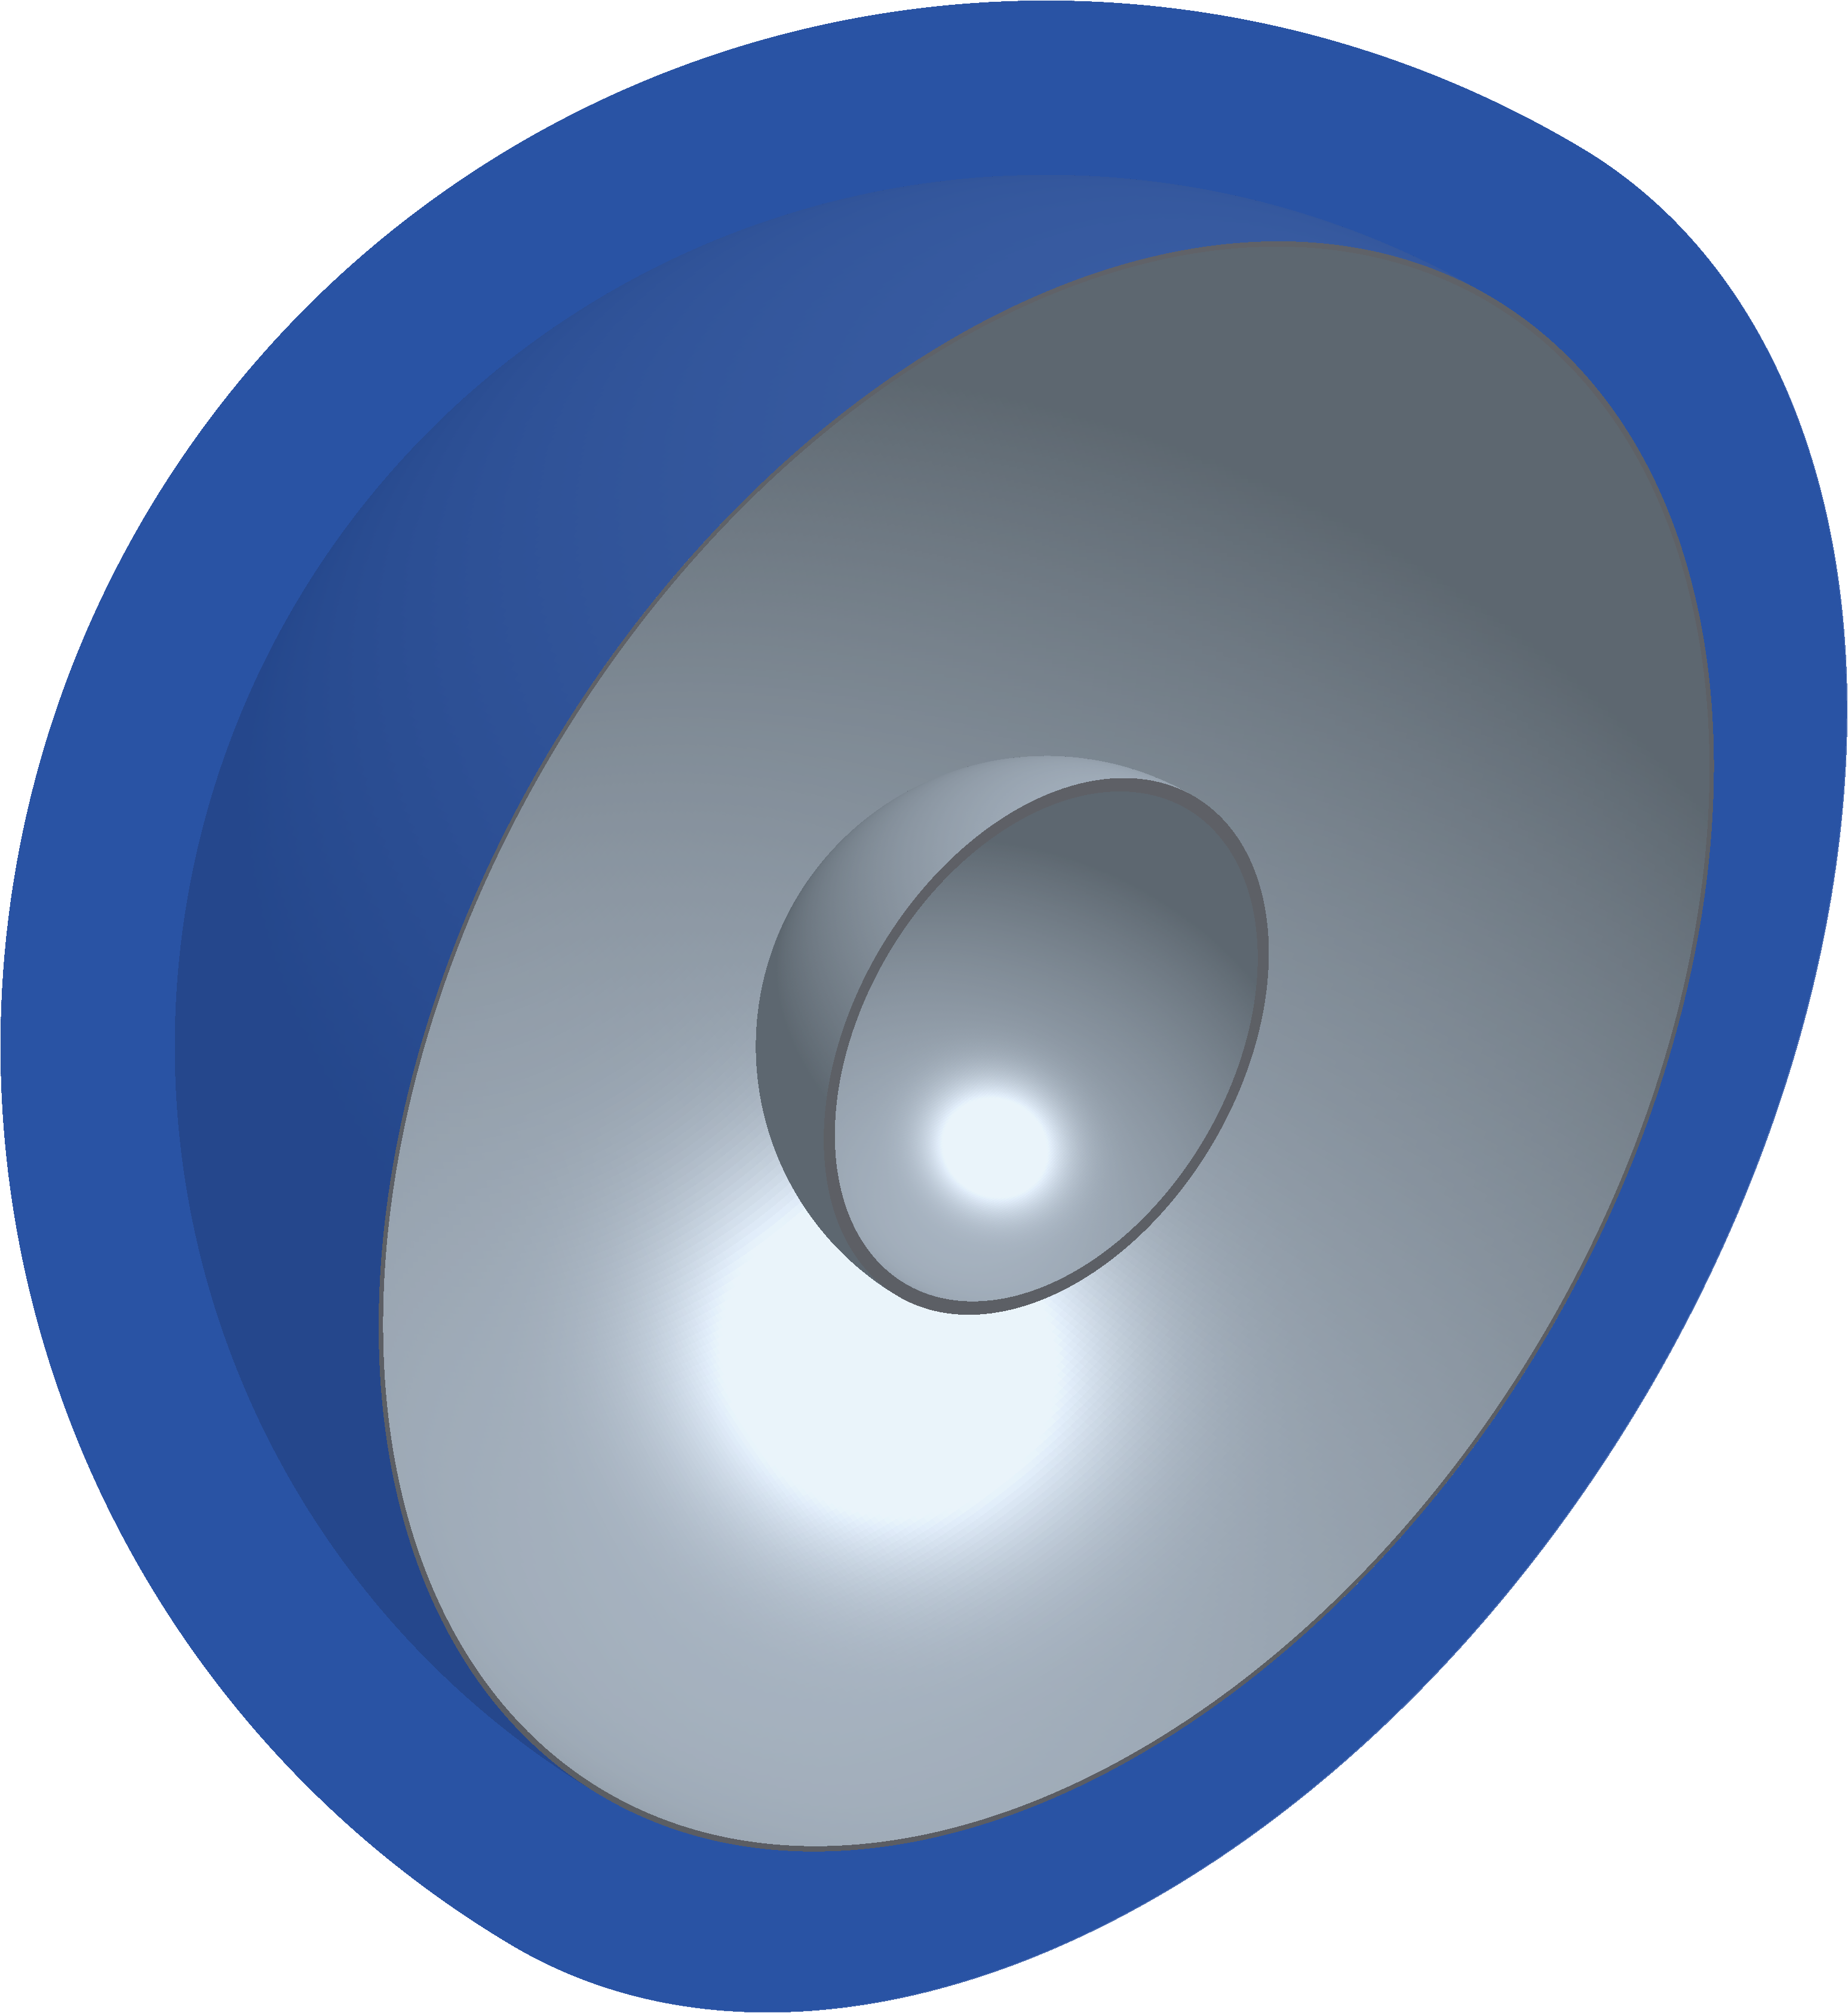
\includegraphics[width=0.8\textwidth]{../../graphics/sphericalShell/half_S13}
		\caption{S13}
    \end{subfigure}
	~
	\begin{subfigure}{0.3\textwidth}
		\centering
%		\includegraphics[width=0.8\textwidth]{\graphicsFolder/Figure15e}
		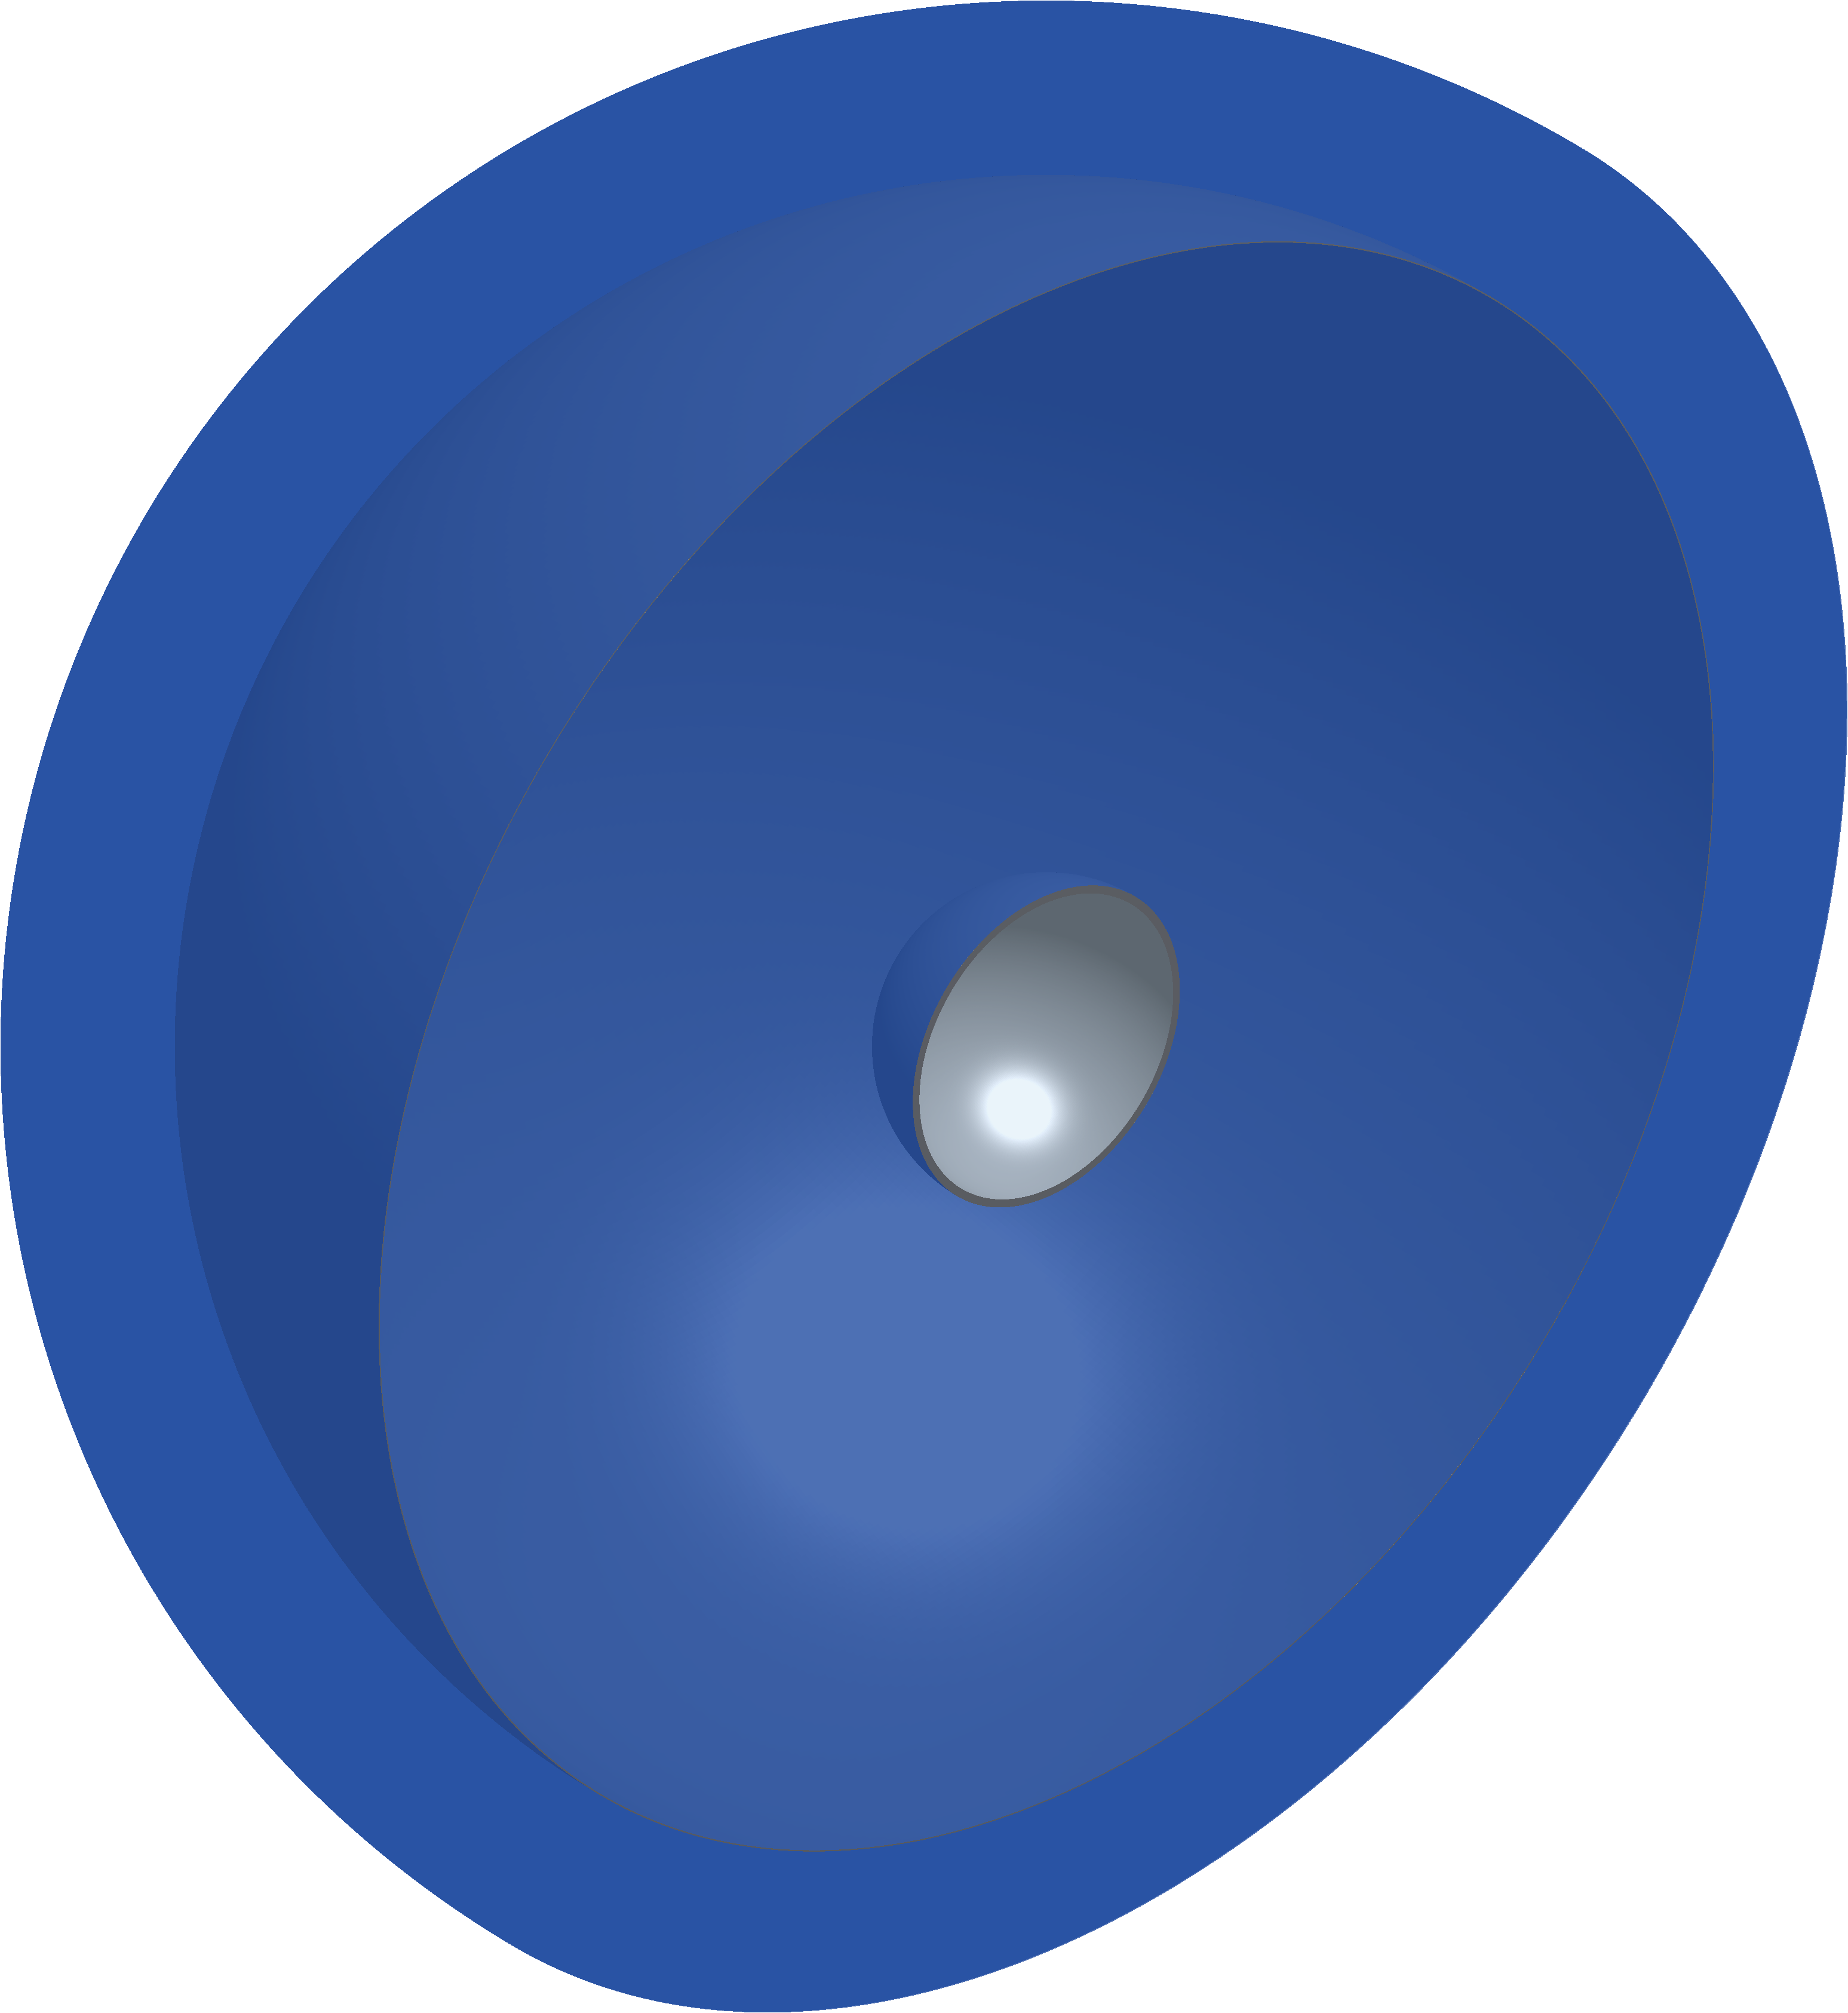
\includegraphics[width=0.8\textwidth]{../../graphics/sphericalShell/half_S15}
		\caption{S15}
    \end{subfigure}
	~
	\begin{subfigure}{0.3\textwidth}
		\centering
%		\includegraphics[width=0.8\textwidth]{\graphicsFolder/Figure15f}
		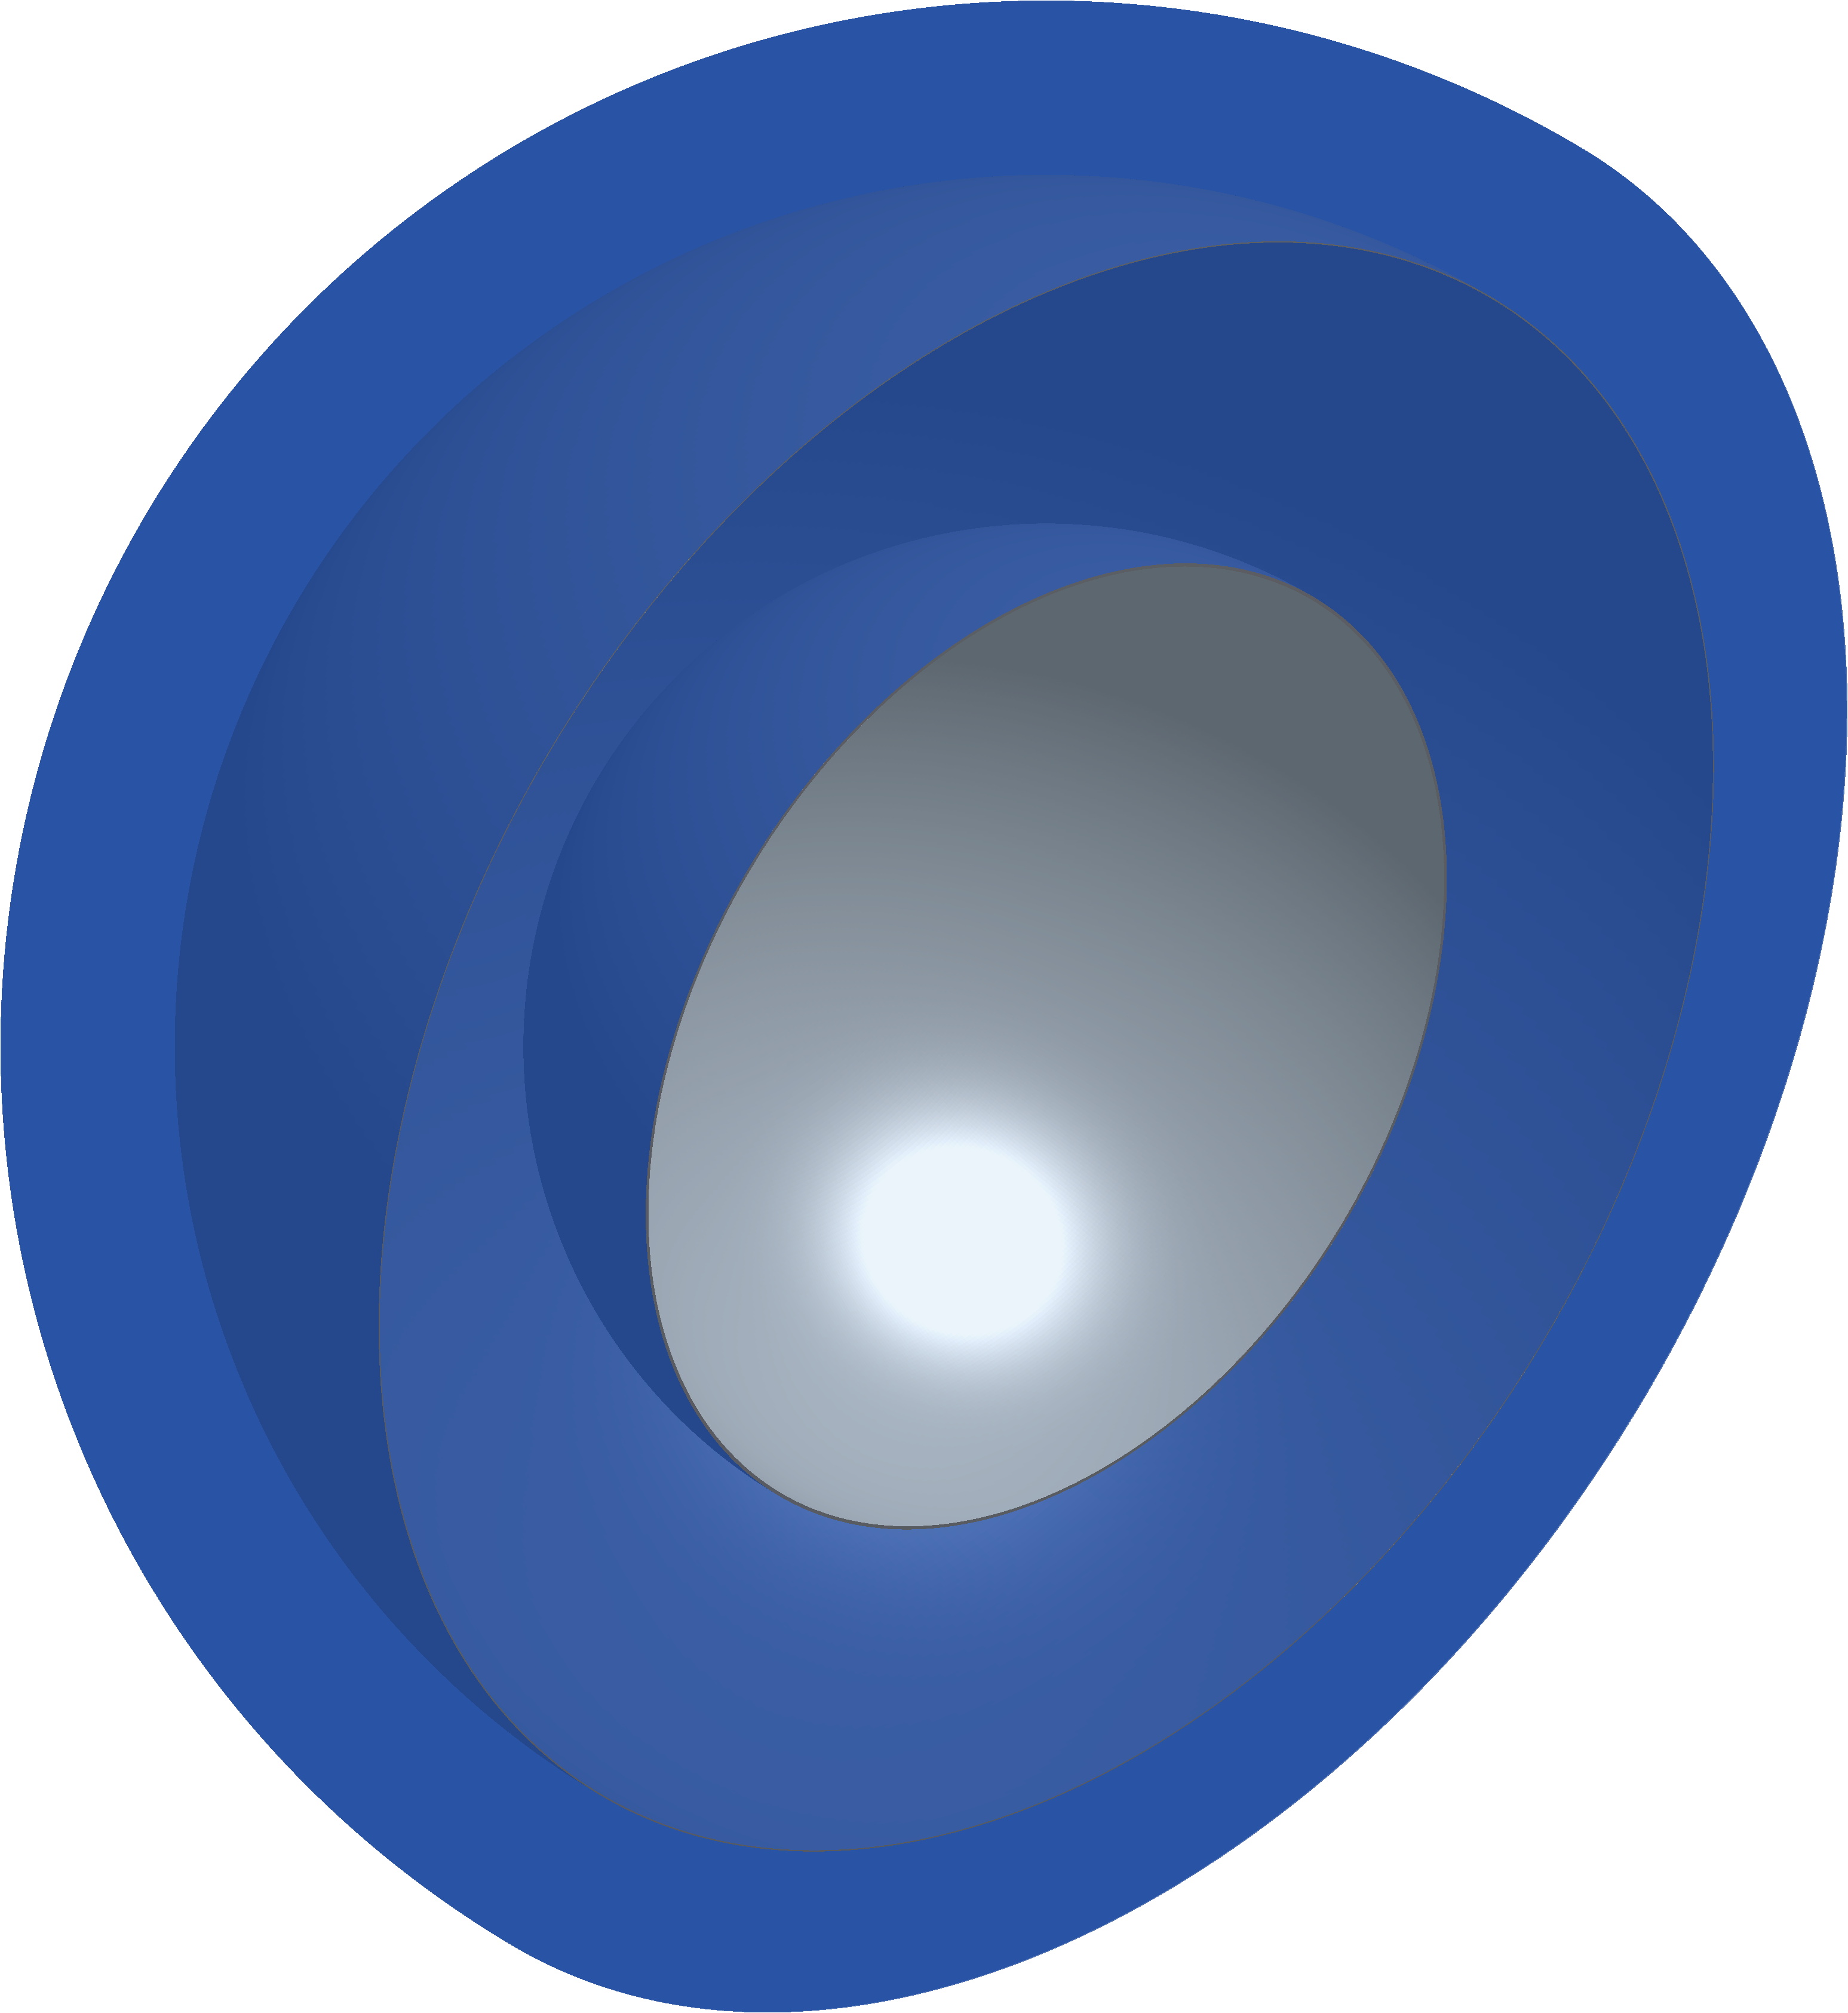
\includegraphics[width=0.8\textwidth]{../../graphics/sphericalShell/half_S35}
		\caption{S35}
    \end{subfigure}
	\par\bigskip
	\begin{subfigure}{0.3\textwidth}
		\centering
%		\includegraphics[width=0.8\textwidth]{\graphicsFolder/Figure15g}
		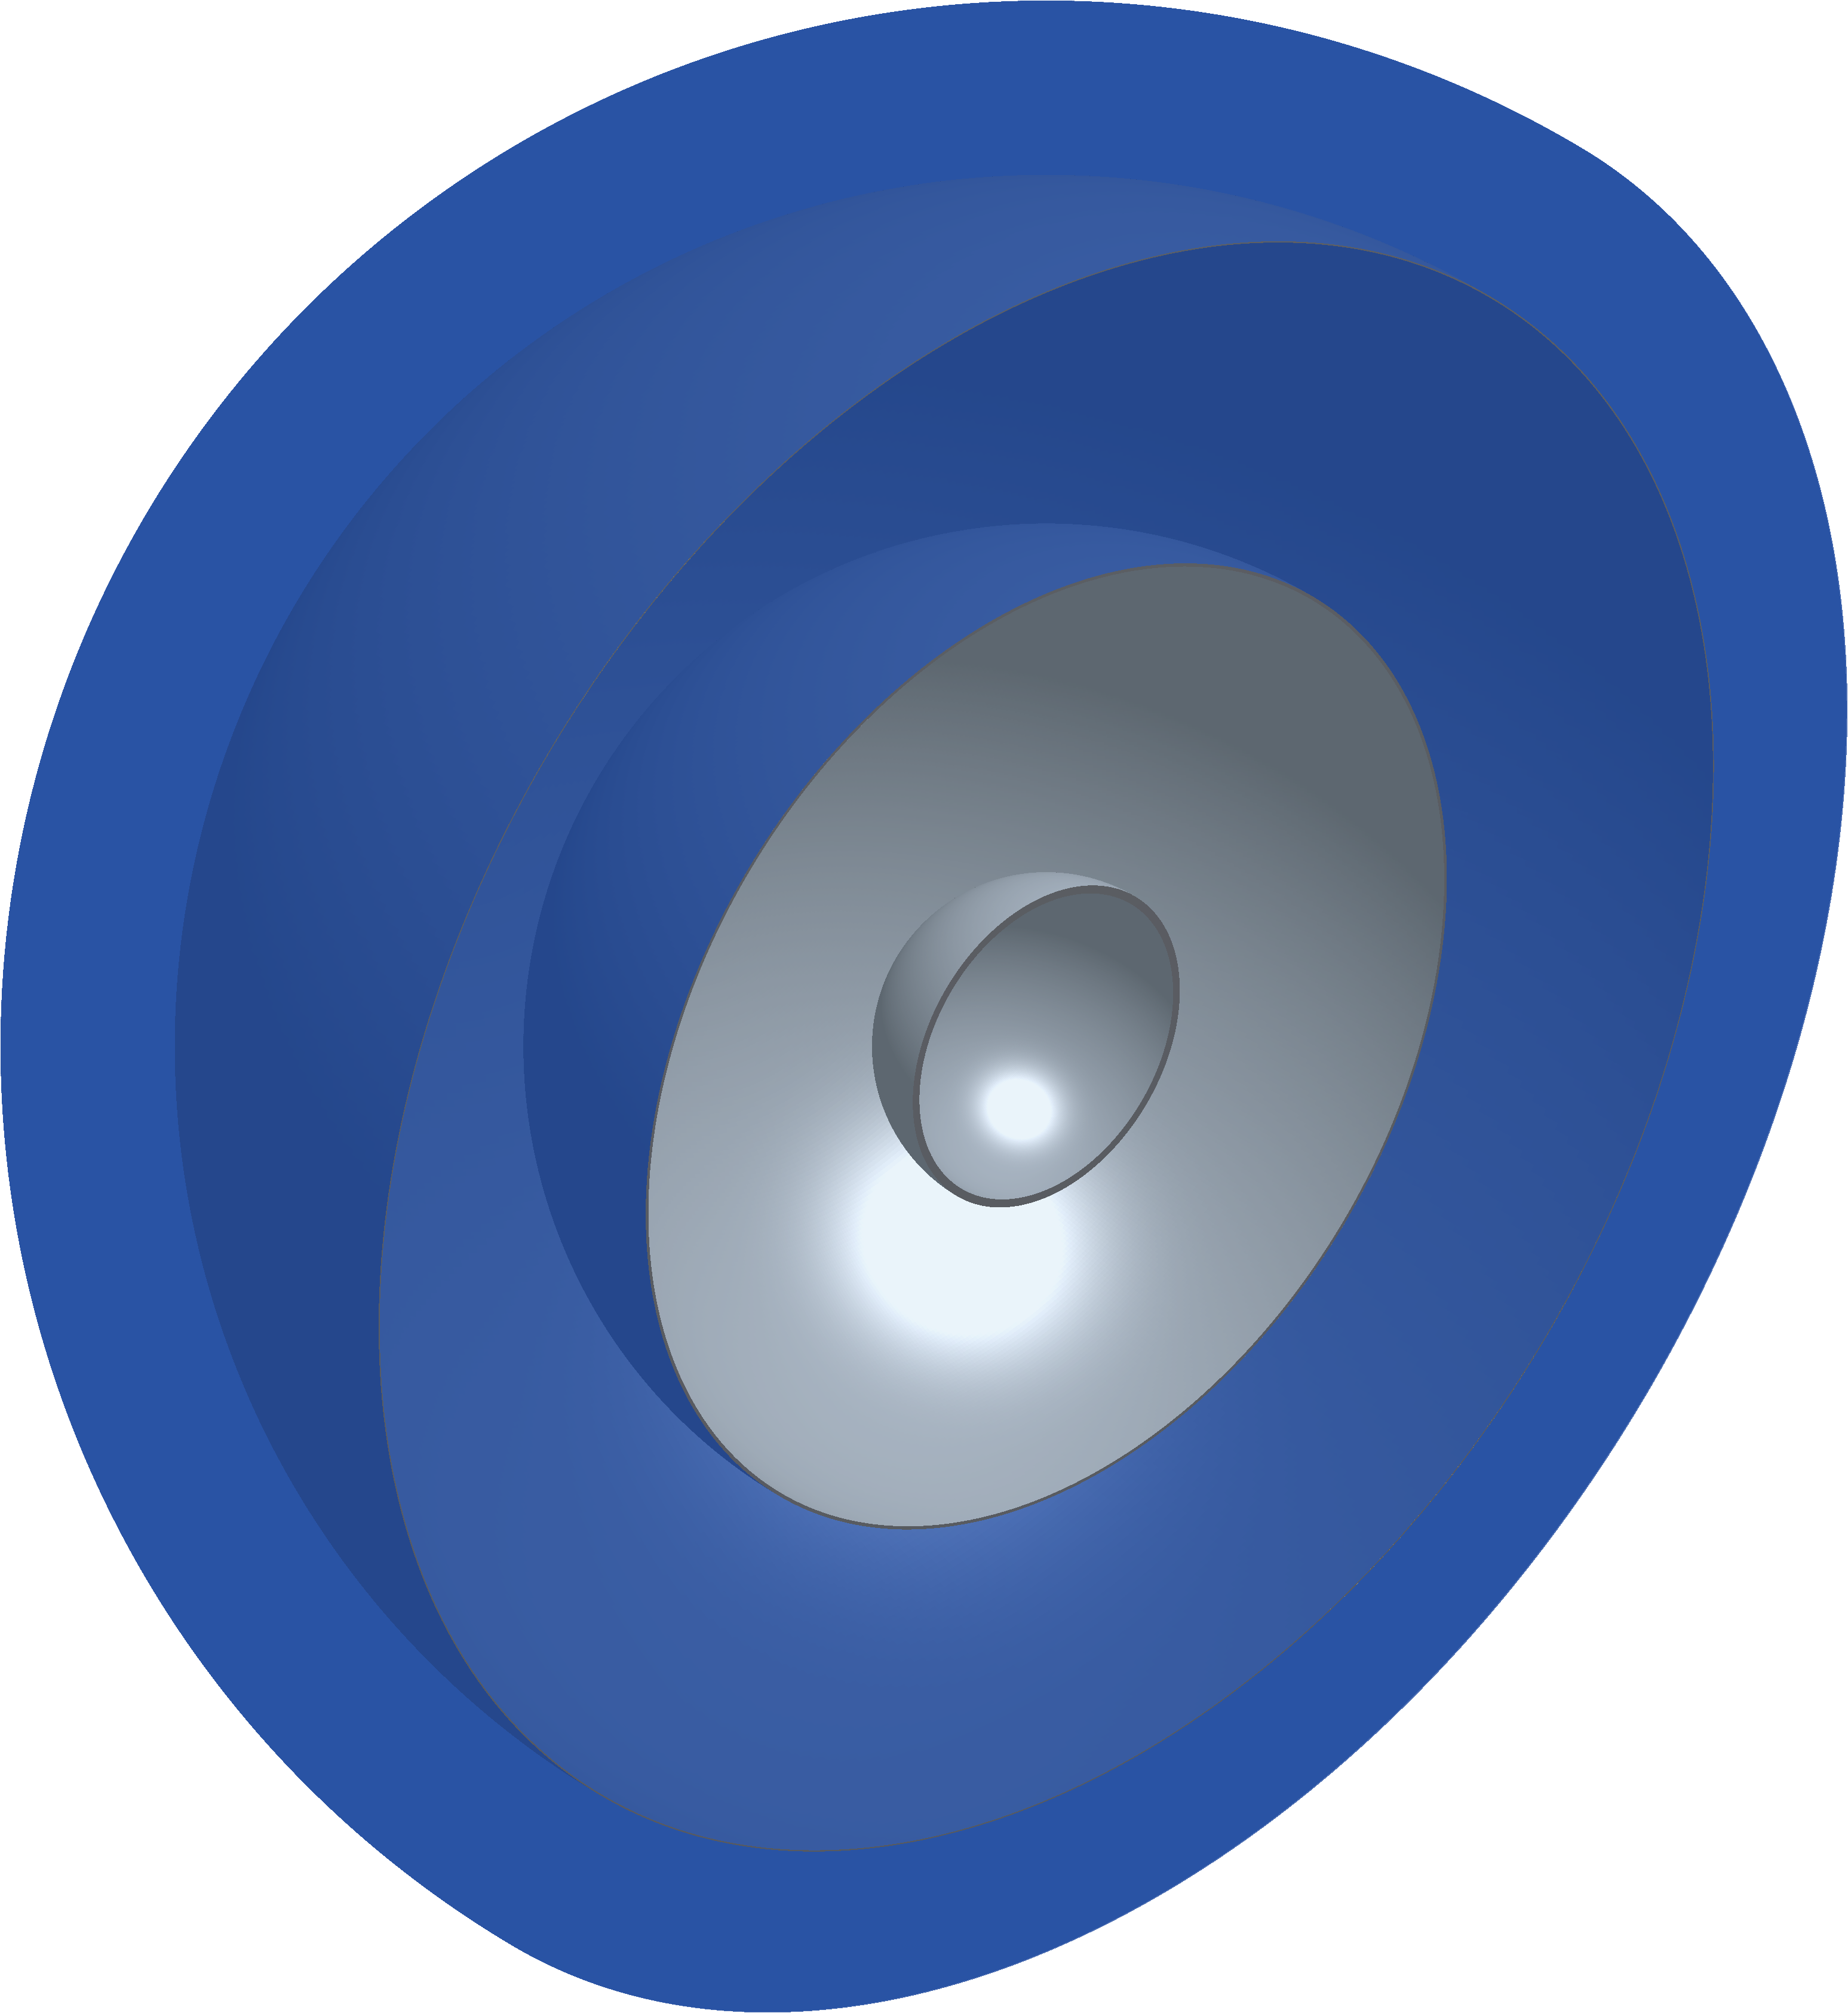
\includegraphics[width=0.8\textwidth]{../../graphics/sphericalShell/half_S135}
		\caption{S135}
    \end{subfigure}
	~
	\begin{subfigure}{0.3\textwidth}
		\centering
%		\includegraphics[width=0.8\textwidth]{\graphicsFolder/Figure15h}
		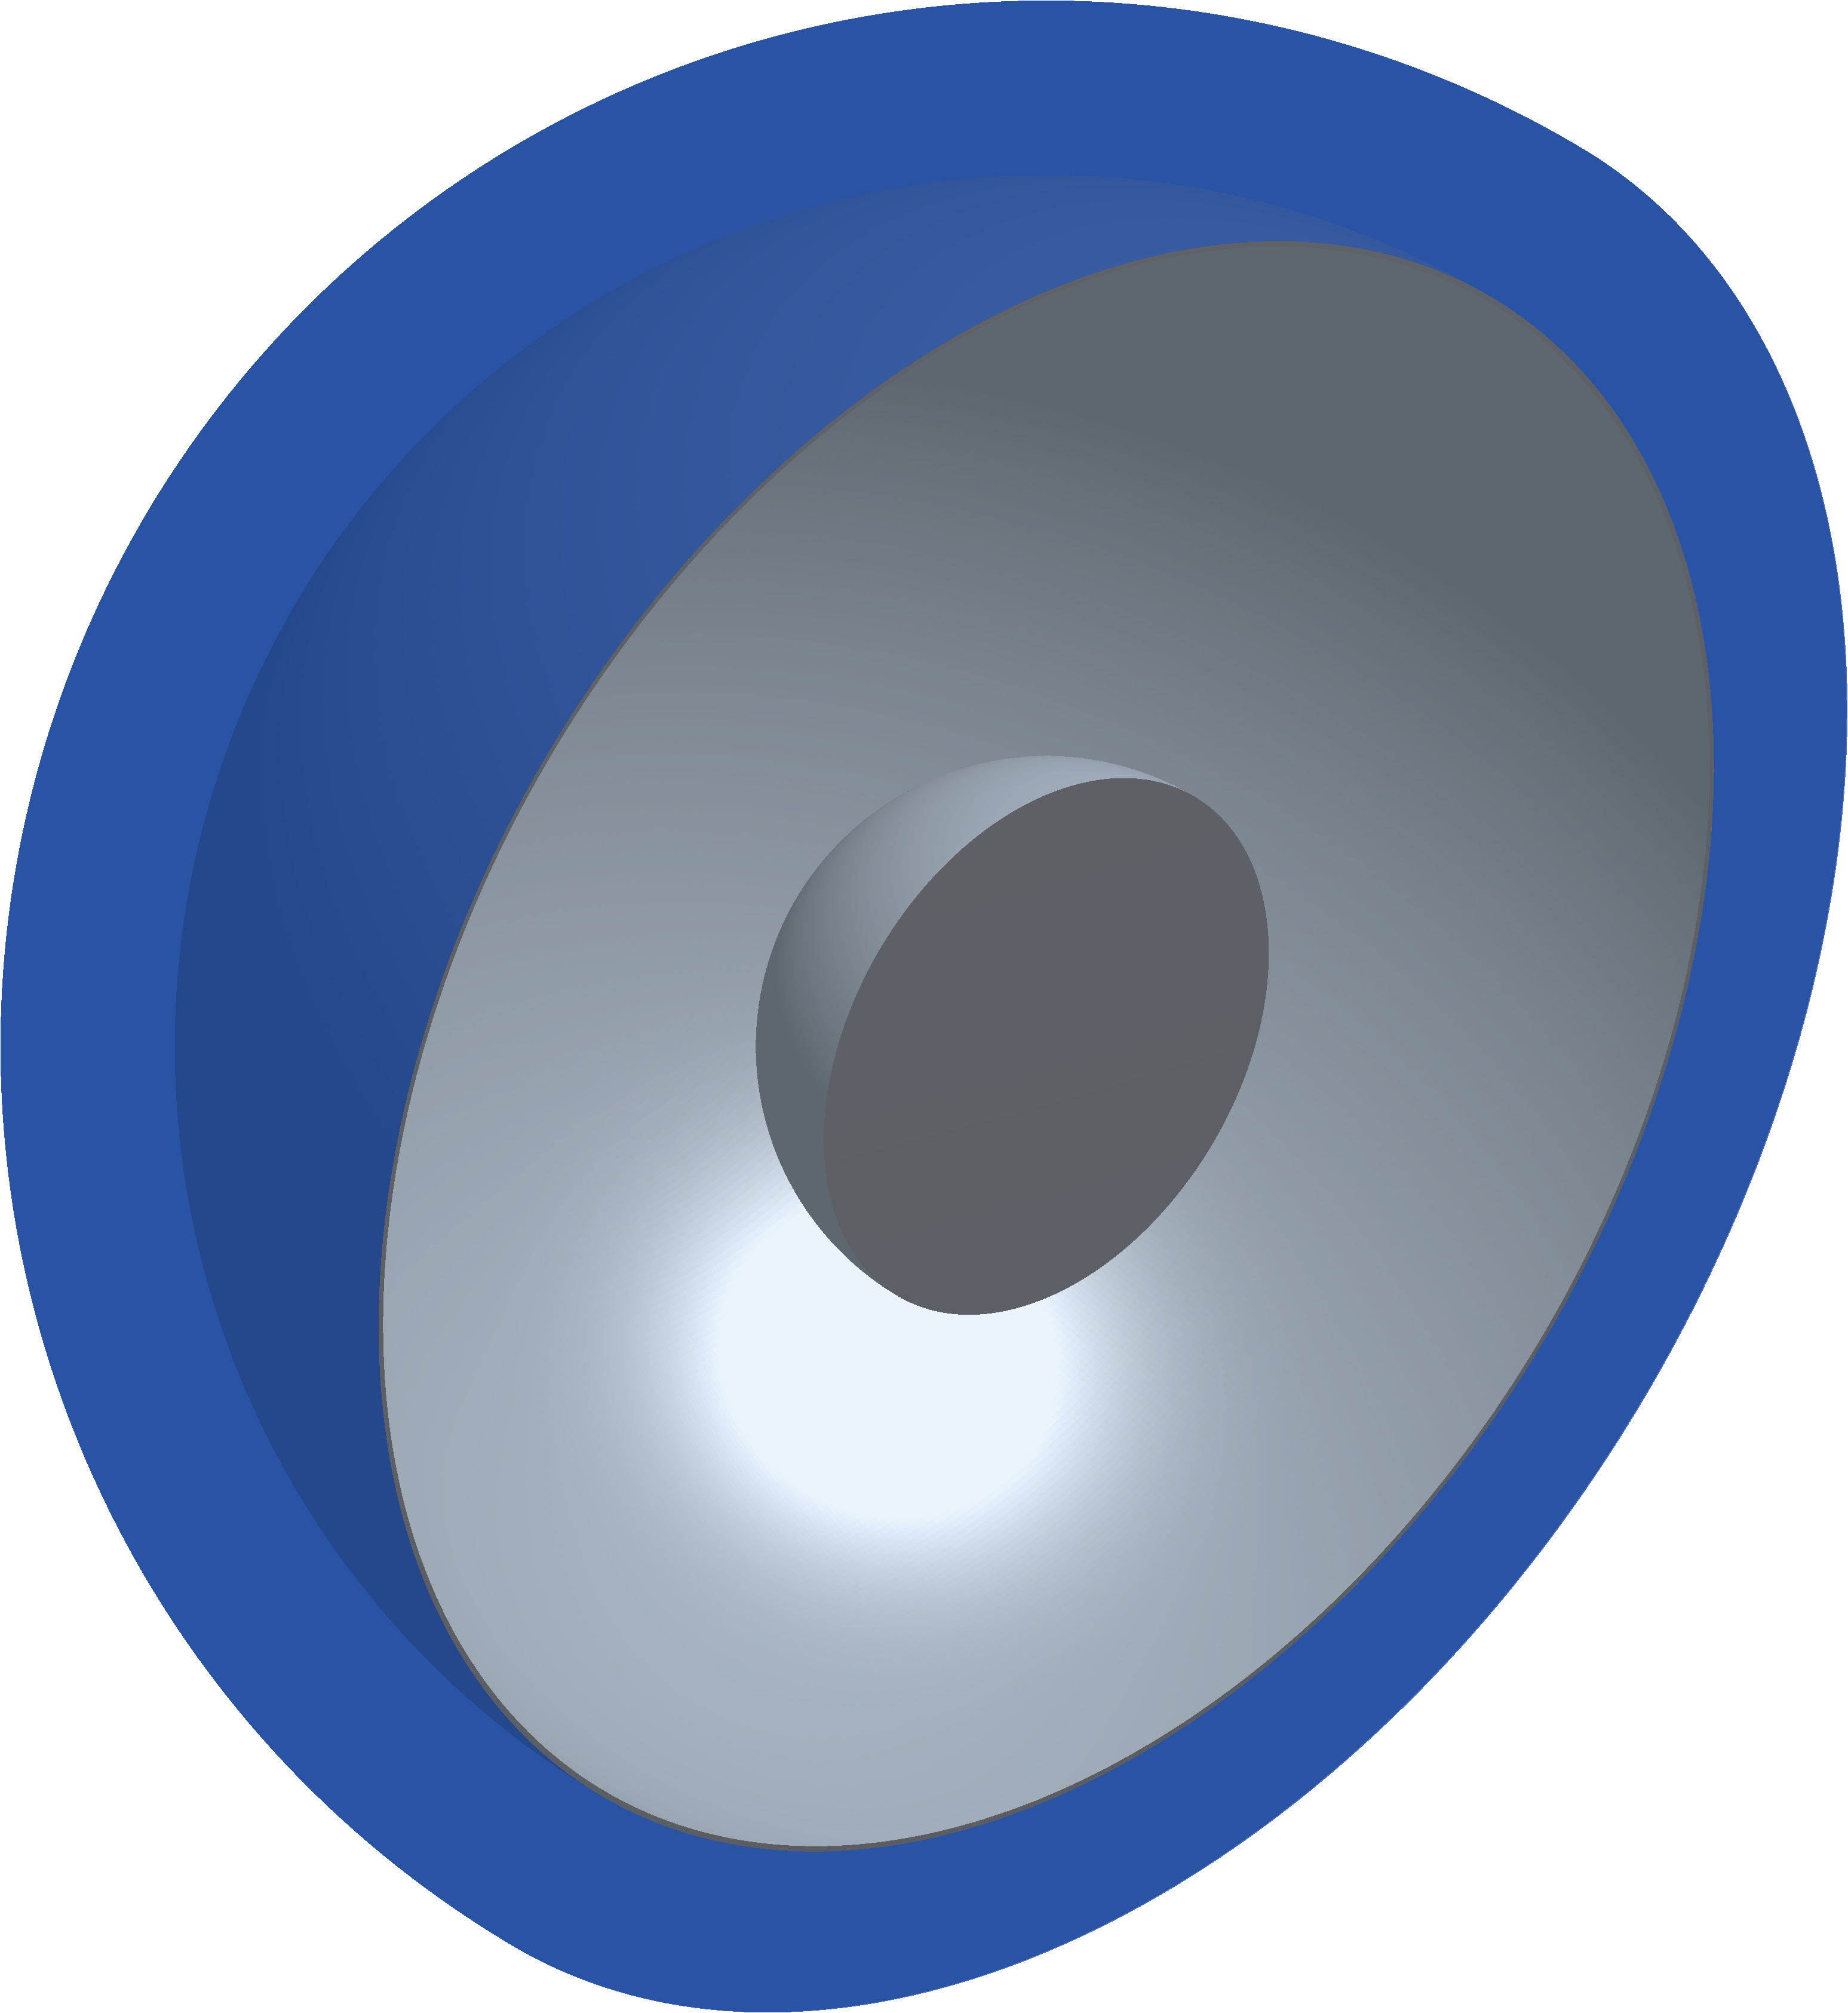
\includegraphics[width=0.8\textwidth]{../../graphics/sphericalShell/S13_ESBC}
		\caption{S13 with ESBC}
		\label{Fig1:S12_ASI_3NN}
    \end{subfigure}
	~
	\begin{subfigure}{0.3\textwidth}
		\centering
%		\includegraphics[width=0.8\textwidth]{\graphicsFolder/Figure15i}
		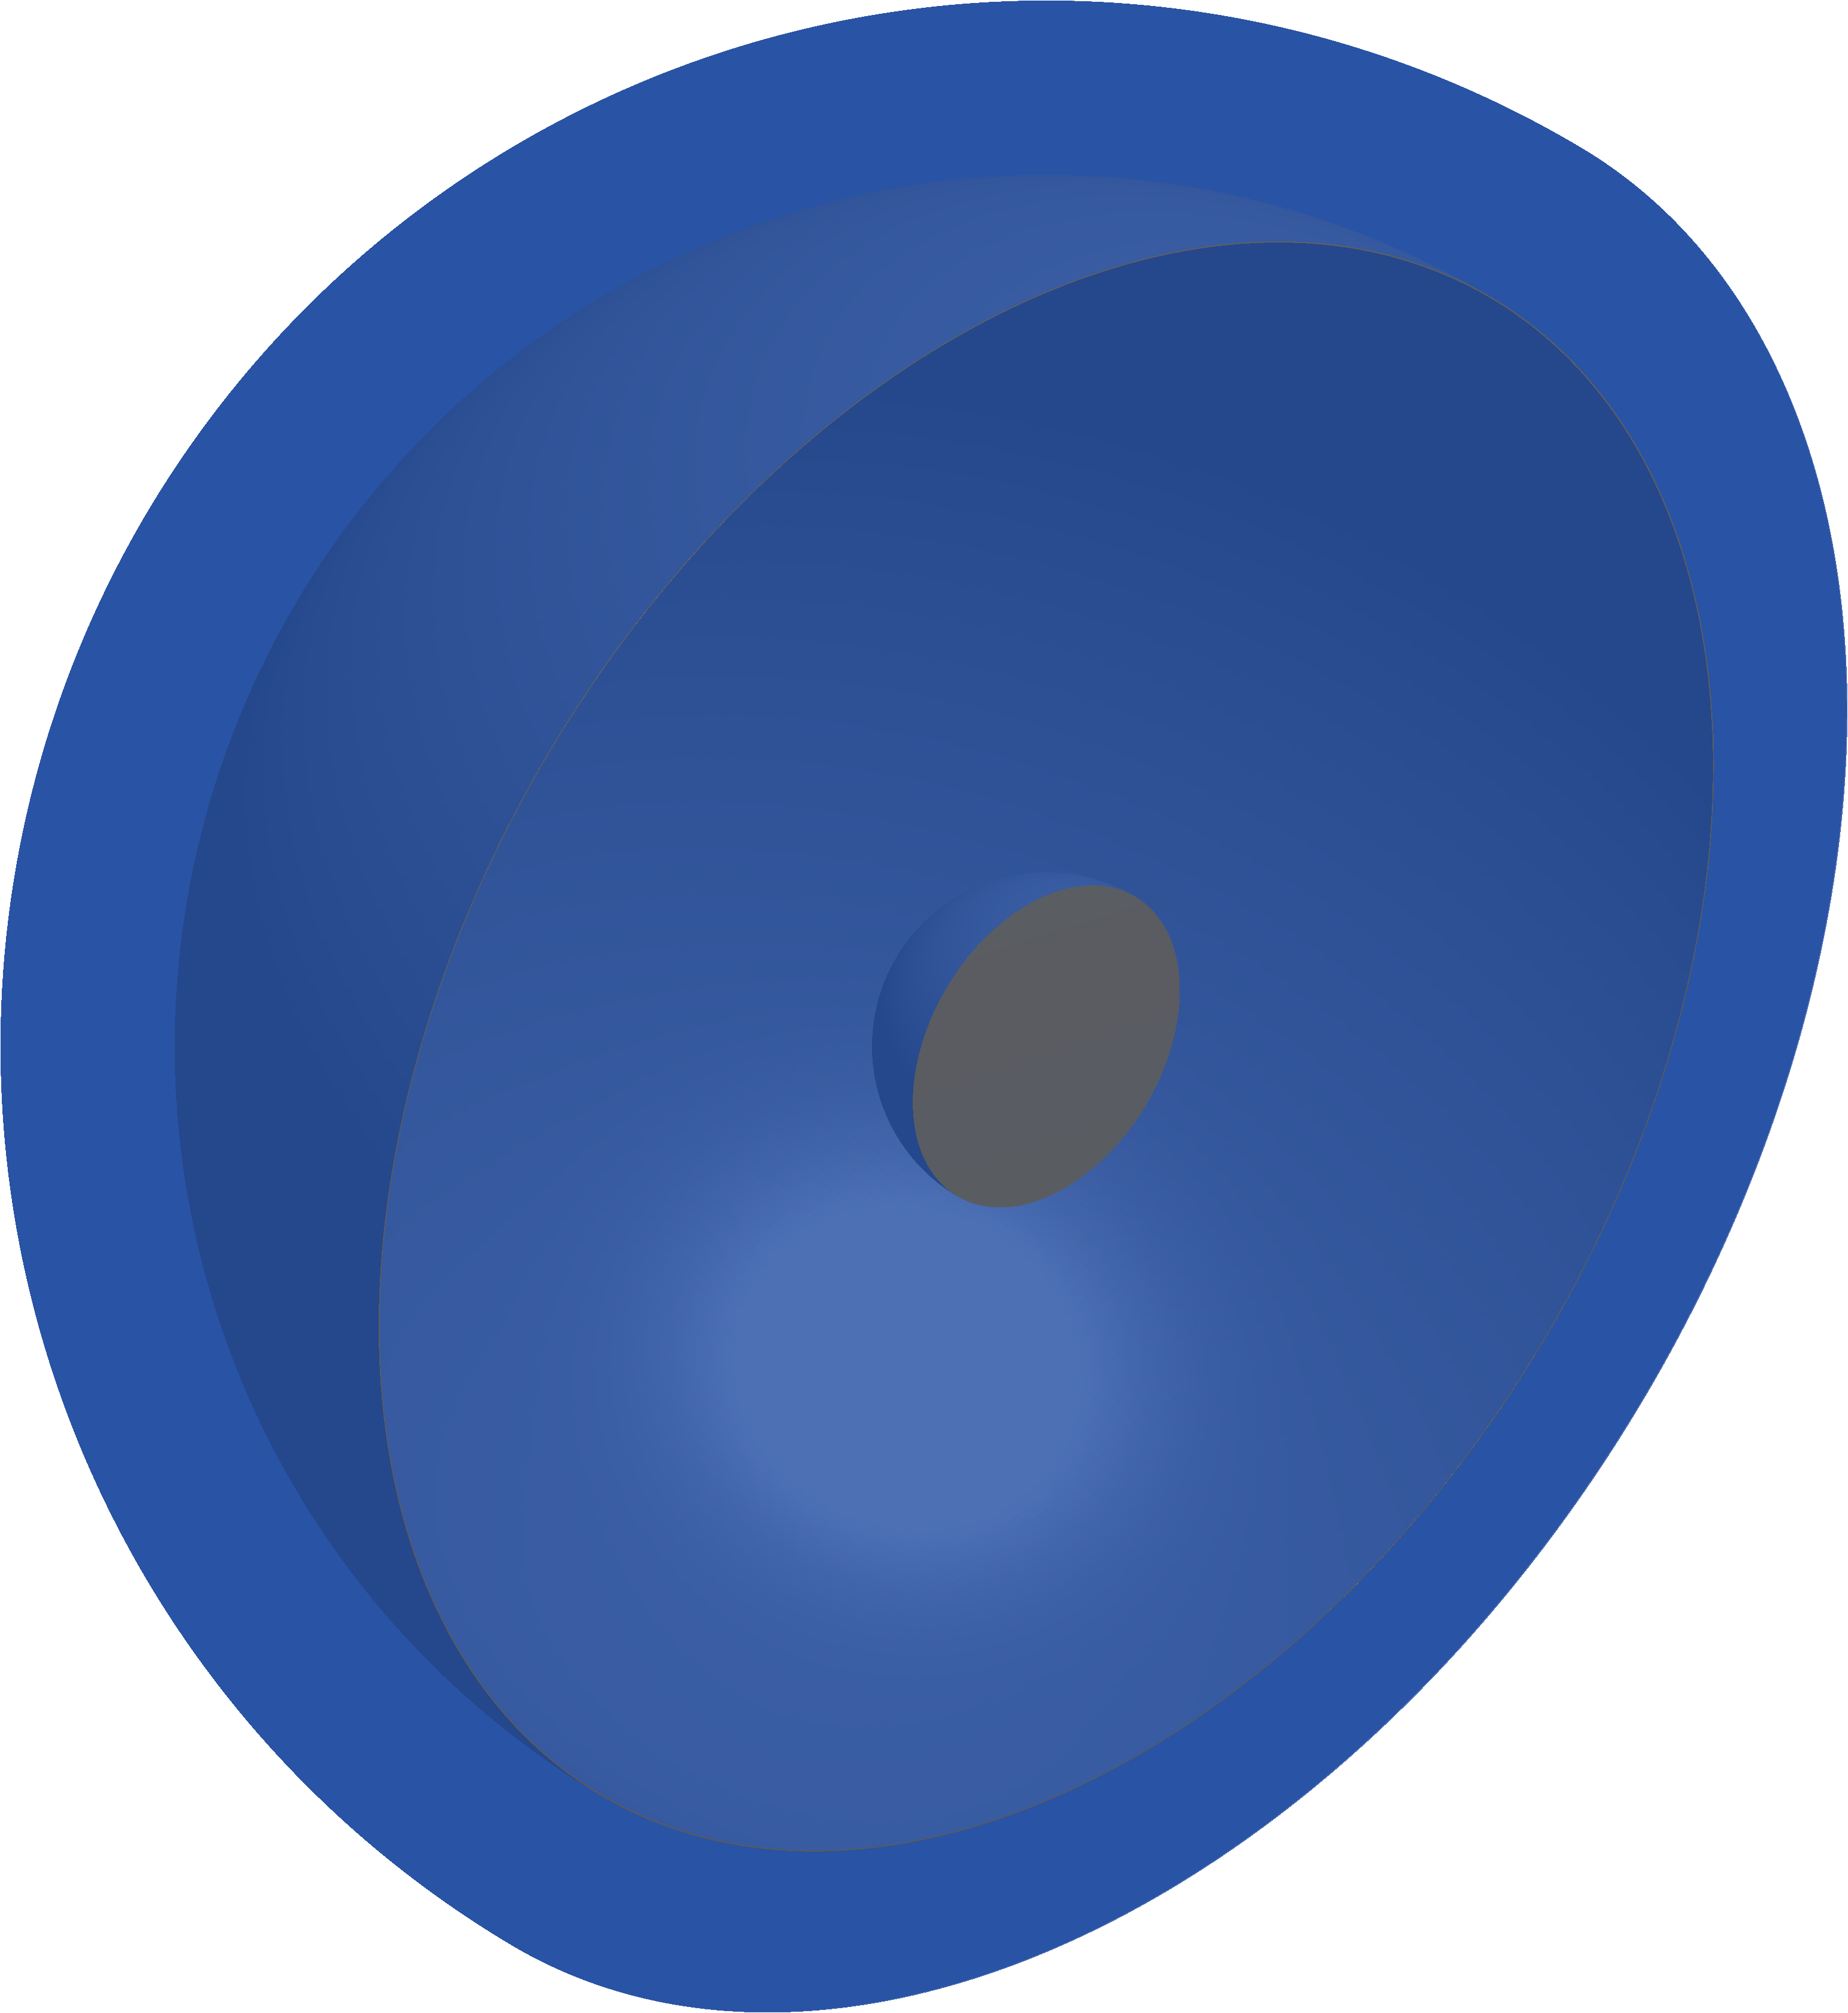
\includegraphics[width=0.8\textwidth]{../../graphics/sphericalShell/S15_ESBC}
		\caption{S15 with ESBC}
		\label{Fig1:S23_ASI_3NN}
    \end{subfigure}
    \caption{\textbf{Benchmark problems}: The first row (S1, S2, S3) represent the default set of benchmarks from which the others are built (clip view). The model S5 and S3 is, respectively, 5 and 3 times the size of S1 (the figures are thus not to scale). S13 is a combination of S1 and S2, S13 is a combination of S1 and S3, and S23 is a combination of S2 and S3. S123 is a combination of S1, S2 and S3. The final two figures are derived models with a solid sphere as the innermost domain.}
	\label{Fig1:BenchmarksProblems}
\end{figure}

By default, all benchmarks have acoustic structure interaction (ASI) on all of the interfaces between fluid and solid domains (with Neumann-to-Neumann boundary conditions, NNBC, in \Cref{Eq1:firstBC,Eq1:secondBC}). As described in \Cref{Subsec1:alternativeBoundaryConditions}, the boundary conditions on the innermost shell may be replaced by other boundary conditions like the sound-soft (SSBC) and sound-hard boundary condition (SHBC). The elastic sphere boundary condition (ESBC) results from filling the innermost shell with the given elastic material. 

In \Cref{Fig1:Benchmarks_NearField}, the near field is plotted for some of these benchmarks. In \Cref{Fig1:S5_SHBC_abs} the classical interference pattern emerging behind the rigid scatterer S5 (with SHBC) can be observed. In contrast, the corresponding case with NNBC in \Cref{Fig1:S5_NNBC_real,Fig1:S5_NNBC_abs} gives a different picture entirely because most of the energy simply passes straight through the thin spherical shell. The example is expanded further in \Cref{Fig1:S35_SHBC_real,Fig1:S35_SHBC_abs,Fig1:S35_NNBC_real,Fig1:S35_NNBC_abs}. For the latter case, the energy transmitted is greatly reduced due to air-filled fluid inside the second shell. The S135 benchmark was visually identical to this benchmark due to this fact (that is, it is hard to reveal objects inside air-filled domains). However, it is clear that sound-hard boundary conditions are not a good approximation of NNBC in this case. The more natural approximation would be to use SSBC. Indeed, the SSBC approximate the innermost fluid with $p_{M+1}=0$, which is clearly a good approximation in this case.
\begin{figure}
	\centering
	\begin{subfigure}[t]{0.49\textwidth}
		\centering
		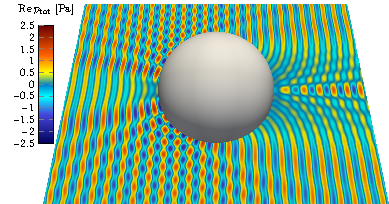
\includegraphics{../../LaTeX/createFigures/TikzFigures/article_e3Dss_PhD/nearFields_S5_SHBC_real}
%		\includegraphics{\graphicsFolder/Figure16a}
		\caption{\textbf{S5 with SHBC}: Plot of $\Re p_{\mathrm{tot}}$.}
		\label{Fig1:S5_SHBC_real}
	\end{subfigure}%
	\hspace*{0.02\textwidth}%
	\begin{subfigure}[t]{0.49\textwidth}
		\centering
		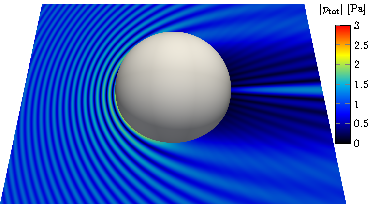
\includegraphics{../../LaTeX/createFigures/TikzFigures/article_e3Dss_PhD/nearFields_S5_SHBC_abs}
%		\includegraphics{\graphicsFolder/Figure16b}
		\caption{\textbf{S5 with SHBC}: Plot of $|p_{\mathrm{tot}}|$.}
		\label{Fig1:S5_SHBC_abs}
	\end{subfigure}%
	\par\bigskip
	\begin{subfigure}[t]{0.49\textwidth}
		\centering
		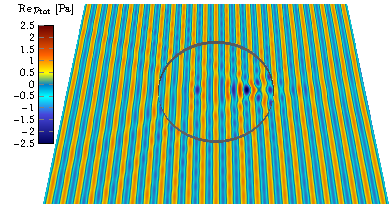
\includegraphics{../../LaTeX/createFigures/TikzFigures/article_e3Dss_PhD/nearFields_S5_NNBC_real}
%		\includegraphics{\graphicsFolder/Figure16c}
		\caption{\textbf{S5 with NNBC}: Plot of $\Re p_{\mathrm{tot}}$.}
		\label{Fig1:S5_NNBC_real}
	\end{subfigure}%
	\hspace*{0.02\textwidth}%
	\begin{subfigure}[t]{0.49\textwidth}
		\centering
		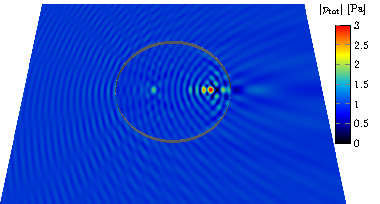
\includegraphics{../../LaTeX/createFigures/TikzFigures/article_e3Dss_PhD/nearFields_S5_NNBC_abs}
%		\includegraphics{\graphicsFolder/Figure16d}
		\caption{\textbf{S5 with NNBC}: Plot of $|p_{\mathrm{tot}}|$.}
		\label{Fig1:S5_NNBC_abs}
	\end{subfigure}%
	\par\bigskip
	\begin{subfigure}[t]{0.49\textwidth}
		\centering
		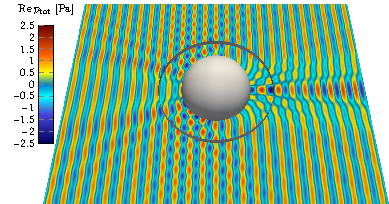
\includegraphics{../../LaTeX/createFigures/TikzFigures/article_e3Dss_PhD/nearFields_S35_SHBC_real}
%		\includegraphics{\graphicsFolder/Figure16e}
		\caption{\textbf{S35 with SHBC}: Plot of $\Re p_{\mathrm{tot}}$.}
		\label{Fig1:S35_SHBC_real}
	\end{subfigure}%
	\hspace*{0.02\textwidth}%
	\begin{subfigure}[t]{0.49\textwidth}
		\centering
		\includegraphics{../../LaTeX/createFigures/TikzFigures/article_e3Dss_PhD/nearFields_S35_SHBC_abs}
%		\includegraphics{\graphicsFolder/Figure16f}
		\caption{\textbf{S35 with SHBC}: Plot of $|p_{\mathrm{tot}}|$.}
		\label{Fig1:S35_SHBC_abs}
	\end{subfigure}%
	\par\bigskip
	\begin{subfigure}[t]{0.49\textwidth}
		\centering
		\includegraphics{../../LaTeX/createFigures/TikzFigures/article_e3Dss_PhD/nearFields_S35_NNBC_real}
%		\includegraphics{\graphicsFolder/Figure16g}
		\caption{\textbf{S135 with NNBC}: Plot of $\Re p_{\mathrm{tot}}$.}
		\label{Fig1:S35_NNBC_real}
	\end{subfigure}%
	\hspace*{0.02\textwidth}%
	\begin{subfigure}[t]{0.49\textwidth}
		\centering
		\includegraphics{../../LaTeX/createFigures/TikzFigures/article_e3Dss_PhD/nearFields_S35_NNBC_abs}
%		\includegraphics{\graphicsFolder/Figure16h}
		\caption{\textbf{S135 with NNBC}: Plot of $|p_{\mathrm{tot}}$.}
		\label{Fig1:S35_NNBC_abs}
	\end{subfigure}%
	\caption{\textbf{Benchmark problems}: Plots of the near field of some benchmark problems. The shells are cut open whenever a domain inside the shell is present. The visualization was done in \href{http://www.paraview.org/}{Paraview}.}
	\label{Fig1:Benchmarks_NearField}
\end{figure}

\subsection{Benchmark problems in the time domain}
Finally, the application of the work in the time domain will be presented. In particular, consider scattering by a single wavelet given by (from~\cite[p. 633]{Jensen2011coa})
\begin{equation}\label{Eq1:Pb_inc}
	\breve{P}_{\mathrm{inc}}(t) = \begin{cases} \frac{4}{3\sqrt{3}} \left[\sin(\omega_{\mathrm{c}} t)-\frac12 \sin\left(2\omega_{\mathrm{c}} t\right)\right] & 0 < t < \frac{1}{f_{\mathrm{c}}}\\
	0 & \text{otherwise},\end{cases}
\end{equation}
with $\omega_{\mathrm{c}} = 2\PI f_{\mathrm{c}}$ and $k_{\mathrm{c}} = \omega_{\mathrm{c}}/c_{\mathrm{f},1}$, and where $f_{\mathrm{c}}$ is the center frequency  (\Cref{Fig1:Pb_inc}). The corresponding frequency spectrum (using the definition of the Fourier transform in \Cref{Eq1:Psi}), is given by (\Cref{Fig1:P_inc})
\begin{figure}
	\centering
	\begin{subfigure}[t]{0.48\textwidth}
		\centering
		\includegraphics{../../LaTeX/createFigures/TikzFigures/article_e3Dss_PhD/P_inc_1}
%		\includegraphics{\graphicsFolder/Figure17a}
		\caption{Wavelet in time domain.}
		\label{Fig1:Pb_inc}
	\end{subfigure}
	~
	\begin{subfigure}[t]{0.48\textwidth}
		\centering
		\includegraphics{../../LaTeX/createFigures/TikzFigures/article_e3Dss_PhD/P_inc_2}
%		\includegraphics{\graphicsFolder/Figure17b}
		\caption{Wavelet in frequency domain.}
		\label{Fig1:P_inc}
	\end{subfigure}
	\caption{\textbf{Benchmark problems in the time domain}: Wavelet $\breve{P}_{\mathrm{inc}}(t)$ and corresponding frequency spectrum $|P_{\mathrm{inc}}(\omega)|$. The wavelet has compact support on the interval $[0,1/f_{\mathrm{c}}]$, where $f_{\mathrm{c}}=\SI{1.5e3}{Hz}$. The frequency spectrum is plotted for positive frequencies to the end of the bandwidth, $f=B/2=\SI{6.4e3}{Hz}$ (with $B=\check{N}/T$).}
\end{figure}
\begin{equation}
	P_{\mathrm{inc}}(\omega) = \left(\fourier\breve{P}_{\mathrm{inc}}\right)(\omega) = \begin{cases}
		\frac{4}{3\sqrt{3}}\frac{\imag\PI}{\omega}\euler^{\imag\PI\omega/\omega_{\mathrm{c}}} & \omega \in\{\pm\omega_{\mathrm{c}},\pm 2\omega_{\mathrm{c}}\}\\
		\frac{4}{\sqrt{3}}\frac{\omega_{\mathrm{c}}^3}{\left(\omega^2-\omega_{\mathrm{c}}^2\right)\left(\omega^2-4\omega_{\mathrm{c}}^2\right)}\left(1-\euler^{-2\PI\imag\omega/\omega_{\mathrm{c}}}\right) & \text{otherwise.}
		\end{cases}
\end{equation}
A plane wave with this wavelet in the time-domain then takes the form
\begin{equation}\label{Eq1:PlaneWaveTimeDomain}
	\breve{p}_{\mathrm{inc}}(\vec{x},t) = \breve{P}_{\mathrm{inc}}\left(t-\frac{x_3}{c_{\mathrm{f},1}}\right),
\end{equation}
with corresponding field in the frequency domain given by
\begin{equation}
	p_{\mathrm{inc}}(\vec{x},\omega)=\left(\fourier\breve{p}_{\mathrm{inc}}(\vec{x},\cdot)\right)(\omega) = P_{\mathrm{inc}}(\omega)\euler^{\imag k_1 x_3}.
\end{equation}
%Alternatively one could use
%\begin{equation*}
%\breve{P}_{\mathrm{inc}}(t) = \begin{cases} \frac{1}{2} \left[-\cos(\omega_{\mathrm{c}} t)+\cos\left(2\omega_{\mathrm{c}} t\right)\right] & 0 < t < \frac{1}{f_{\mathrm{c}}}\\
%	0 & \text{otherwise}\end{cases}
%\end{equation*}
%with the frequency spectrum
%\begin{equation*}
%	P_{\mathrm{inc}}(\omega) =  \begin{cases}
%		\frac{\PI}{2\omega_{\mathrm{c}}}\euler^{\imag\PI\omega/\omega_{\mathrm{c}}} & \omega \in\{\pm\omega_{\mathrm{c}},\pm 2\omega_{\mathrm{c}}\}\\
%		-\frac{3}{2}\frac{\imag\omega\omega_{\mathrm{c}}^2}{\left(\omega^2-\omega_{\mathrm{c}}^2\right)\left(\omega^2-4\omega_{\mathrm{c}}^2\right)}\left(1-\euler^{-2\PI\imag\omega/\omega_{\mathrm{c}}}\right) & \text{otherwise.}
%		\end{cases}
%\end{equation*}
An alternative to plane waves, is waves due to point sources. Using the wavelet in \Cref{Eq1:Pb_inc}, these waves are given by
\begin{equation}
	\breve{p}_{\mathrm{inc}}(\vec{x},t) = \breve{P}_{\mathrm{inc}}\left(t-\frac{|\vec{x}_{\mathrm{s}}-\vec{x}|}{c_{\mathrm{f},1}}\right)\frac{r_{\mathrm{s}}}{|\vec{x}_{\mathrm{s}}-\vec{x}|}\label{Eq1:P_incOmega}
\end{equation}
and
\begin{equation*}
	p_{\mathrm{inc}}(\vec{x},\omega) = P_{\mathrm{inc}}(\omega)\frac{r_{\mathrm{s}}}{|\vec{x}_{\mathrm{s}}-\vec{x}|}\euler^{\imag k_1 |\vec{x}_{\mathrm{s}}-\vec{x}|}
\end{equation*}
where $\vec{x}_{\mathrm{s}}$ is location of the point source given in \Cref{Eq1:x_s} (at a finite distance $r_{\mathrm{s}}=|\vec{x}_{\mathrm{s}}|$). 

As $\Psi(\vec{x},\omega)$ cannot be computed for infinitely many frequencies, an approximation of the time dependent fields in \Cref{Eq1:Psit} by~\cite[p. 614]{Jensen2011coa} can be used
\begin{equation}
	\breve{\Psi}(\vec{x},t_m) \approx \frac{2}{T}\Re\left\{\sum_{n=1}^{\check{N}/2-1} \Psi(\vec{x},\omega_n)\euler^{-2\PI\imag n m/\check{N}}\right\}
\end{equation}
where
\begin{equation}
	t_m = m\Diff t, \quad \Diff t = \frac{T}{\check{N}}, \quad \omega_n = n\Diff\omega, \quad \Diff\omega = \frac{2\PI}{T}. 
\end{equation}
Note that the contribution from the static case ($n=0$) has not been included as the incident wave, $p_{\mathrm{inc}}(\vec{x},0) = 0$, results in the trivial solution $\Psi(\vec{x},0)=0$. The Fourier series approximation results in periodic time-dependent fields, with period $T$, sampled in the interval $[0,T]$ with $\check{N}$ time steps. The parameter $\check{N}$ also quantifies the number of terms in the Fourier series approximation, such that it also controls the error (aliasing). By choosing $\check{N}$ to be powers of two, the approximation can be very efficiently evaluated by the fast Fourier transformation. 

In \Cref{Fig1:S5_ESBC_planeWave} an example based on the S5 benchmark problem with ESBC is illustrated; An elastic sphere (with parameters given in \Cref{Tab1:sphericalShellParameters}) is impinged by the incident wave in \Cref{Eq1:PlaneWaveTimeDomain}. In this example, the following parameters has been used: $f_{\mathrm{c}}=\SI{1.5}{kHz}$, $\check{N}=2^{10}=1024$ and $T=120/f_{\mathrm{c}}$. In \Cref{Fig1:S5_ESBC_planeWave}, the total pressure is plotted in the fluid, and the von Mises stress given by
\begin{equation}
	\sigma_{\mathrm{v}} =  \sqrt{\frac{(\sigma_{11} - \sigma_{22})^2 + (\sigma_{22} - \sigma_{33})^2 + (\sigma_{11} - \sigma_{33})^2 + 6(\sigma_{23}^2 + \sigma_{13}^2 + \sigma_{12}^2)}{2}} 
\end{equation}
is plotted in the solid domain.

For the benchmark problems, the longitudinal speed and transverse speed in the solid is $c_{\mathrm{s},1}\approx \SI{6001}{ms^{-1}}$ and $c_{\mathrm{s},2}\approx \SI{3208}{ms^{-1}}$, respectively. So since, $c_{\mathrm{s},1}\approx 4c_{\mathrm{f}}$ and $c_{\mathrm{s},2}\approx 2c_{\mathrm{f}}$, the waves traveling through the elastic sphere with the longitudinal wave speed will transmit through the solid 4 times as fast as the waves in the surrounding fluid (this wave correspond to the $1^{\mathrm{st}}$ transmitted wave in \Cref{Fig1:S5_ESBC_planeWave}). Correspondingly for the waves traveling with the transverse wave speed. This can indeed be observed as well, but the amplitude of the transverse wave traveling at the speed $c_{\mathrm{s},1}$ is only about $2\%$ of the amplitude of the incident wave $P_{\mathrm{inc}}$, and is thus barely visible. Much more energy is transmitted through the wave with the transverse wave speed (the amplitude is approximately $14\%$ of $P_{\mathrm{inc}}$).
\begin{figure}
	\centering
	\includegraphics[width=\textwidth]{../../LaTeX/createFigures/TikzFigures/article_e3Dss_PhD/S5_ESBC_planeWave}
%	\includegraphics{\graphicsFolder/Figure18}
    \caption{\textbf{Benchmark problems in the time domain}: Visualization of a wavelet (from a far-field point) in the time domain which transmits (the $1^{\mathrm{st}}$ transmitted wave) and reflects (the $1^{\mathrm{st}}$ reflected wave) an elastic sphere (which is cut open for visualization purposes). The $2^{\mathrm{nd}}$ transmitted wave through the elastic sphere takes a lead of the direct wave as the wave speed in the elastic material is larger than that of the fluid. Aliasing is also visible. Two transparent planes have been inserted to visualize the total pressure field. The von Mises stress, $\breve{\sigma}_{\mathrm{v}}$, is visualized in the solid. The visualization was done in \href{http://www.paraview.org/}{Paraview}.}
	\label{Fig1:S5_ESBC_planeWave}
\end{figure}

Consider finally the S15 benchmark problem with ESBC; A thin shell surrounding a solid sphere is impinged by the incident wave in \Cref{Eq1:P_incOmega} (that is, the incident wave originates from a point source in the near field). The point source is located at a radius of $r_{\mathrm{s}}=\SI{10}{m}$ away from the center of the scatterer (the origin). All other parameters remain the same as in the previous example. 

In \Cref{Fig1:S15_ESBC_pointCharge} the effects from previous example can again be observed. In addition, waves traveling in the thin shell are reflected backwards through a head wave in the intermediate fluid. In addition, the corresponding waves are transmitted through the shell denoted as ``Wave from shell''.

It should be pointed out that aliasing (pollution of the solution from the previous incident waves due to periodicity) is present, although not visible in these plots. The aliasing can be decreased further by increasing the period $T$. To preserve the size of the \textit{bandwidth} $B=\check{N}/T$, $\check{N}$ must be correspondingly increased. 
\begin{figure}
	\centering
	\includegraphics[width=\textwidth]{../../LaTeX/createFigures/TikzFigures/article_e3Dss_PhD/S15_ESBC_pointSource}
%	\includegraphics{\graphicsFolder/Figure19}
    \caption{\textbf{Benchmark problems in the time domain}: Visualization of a wavelet (from a point source) in the time domain which transmits (the $1^{\mathrm{st}}$ transmitted wave) and reflects (the $1^{\mathrm{st}}$ reflected wave) the outermost thin shell (which is cut open for visualization purposes), and is then scattered (the $2^{\mathrm{nd}}$ reflected wave) by the innermost solid sphere. The $2^{\mathrm{nd}}$ transmitted wave through the elastic sphere takes a lead of the direct wave as the wave speed in the elastic material is larger than that of the fluid. Aliasing is also visible. Two transparent planes have been inserted to visualize the total pressure field. The displacement field is here not visualized. The visualization was done in \href{http://www.paraview.org/}{Paraview}.}
	\label{Fig1:S15_ESBC_pointCharge}
\end{figure}
%\clearpage